\documentclass[12pt,a4paper]{article}

% ------------------------------- packages ----------------------------------
\usepackage[utf8]{inputenc}
\usepackage[T1]{fontenc}
\usepackage{lmodern}
\usepackage[margin=1in]{geometry}
\usepackage{amsmath,amssymb,amsthm}
\usepackage{mathtools}
\usepackage{microtype}
\usepackage{natbib}
\bibliographystyle{plainnat}
\usepackage[most]{tcolorbox}
\tcbuselibrary{breakable,skins}
\usepackage{hyperref}
\usepackage[nameinlink,capitalize]{cleveref}
\usepackage{enumitem}

% ------- additions from the 8 revised section files -----------------------
\usepackage{tikz}
\usetikzlibrary{positioning,arrows.meta,calc,trees}
\usepackage{pgfplots}
\pgfplotsset{compat=1.17}
\usepackage{booktabs}
\usepackage{xcolor}
\usepackage{eurosym}
\usepackage{listings}
\lstset{
  basicstyle=\ttfamily\small,
  language=Python,
  breaklines=true,
  columns=fullflexible,
  showstringspaces=false,
  frame=single,
  backgroundcolor=\color{gray!5},
  xleftmargin=4pt,
  xrightmargin=4pt,
}

% ------------------------------- theorems ----------------------------------
\theoremstyle{plain}
\newtheorem{theorem}{Theorem}[section]
\newtheorem{lemma}[theorem]{Lemma}
\newtheorem{corollary}[theorem]{Corollary}

\theoremstyle{definition}
\newtheorem{definition}[theorem]{Definition}
\newtheorem{example}[theorem]{Example}

\crefname{theorem}{Theorem}{Theorems}
\crefname{lemma}{Lemma}{Lemmas}
\crefname{corollary}{Corollary}{Corollaries}
\crefname{definition}{Definition}{Definitions}
\crefname{example}{Example}{Examples}
\crefname{section}{Section}{Sections}
\crefname{equation}{Equation}{Equations}

% ------------------------------- boxes -------------------------------------
% intuition box (orange, manager track) -------------------------------------
\newtcolorbox{intuition}[1][]{
  breakable,
  enhanced,
  colback=yellow!8,
  colframe=orange!60!black,
  coltitle=white,
  fonttitle=\bfseries,
  title={Intuition},
  boxrule=0.6pt,
  left=6pt,right=6pt,top=4pt,bottom=4pt,
  #1
}

% activity box (green accent) -----------------------------------------------
\newtcolorbox{activity}[1][]{
  breakable,
  enhanced,
  colback=green!5,
  colframe=green!45!black,
  coltitle=white,
  fonttitle=\bfseries,
  title={Activity},
  boxrule=0.6pt,
  left=6pt,right=6pt,top=4pt,bottom=4pt,
  #1
}

% story box (warm purple) ---------------------------------------------------
\newtcolorbox{story}[1][]{
  breakable,
  enhanced,
  colback=purple!4,
  colframe=purple!55!black,
  coltitle=white,
  fonttitle=\bfseries,
  title={A Short Story},
  boxrule=0.6pt,
  left=6pt,right=6pt,top=4pt,bottom=4pt,
  #1
}

% aside box (grey) ----------------------------------------------------------
\newtcolorbox{aside}[1][]{
  breakable,
  enhanced,
  colback=gray!6,
  colframe=gray!55!black,
  coltitle=white,
  fonttitle=\bfseries,
  title={Aside},
  boxrule=0.5pt,
  left=6pt,right=6pt,top=4pt,bottom=4pt,
  #1
}

% procurement box (teal) ----------------------------------------------------
\newtcolorbox{procurement}[1][]{
  breakable,
  enhanced,
  colback=teal!5,
  colframe=teal!55!black,
  coltitle=white,
  fonttitle=\bfseries,
  title={Procurement corollary},
  boxrule=0.5pt,
  left=6pt,right=6pt,top=3pt,bottom=3pt,
  fontupper=\small,
  #1
}

% decision box (olive/dark green) -------------------------------------------
\newtcolorbox{decisionbox}[1][]{
  breakable,
  enhanced,
  colback=olive!5,
  colframe=olive!55!black,
  coltitle=white,
  fonttitle=\bfseries,
  title={For the decision-maker},
  boxrule=0.6pt,
  left=6pt,right=6pt,top=4pt,bottom=4pt,
  #1
}

% howtoread micro-box (grey, minimal) ---------------------------------------
\newtcolorbox{howtoread}{
  enhanced,
  colback=gray!8,
  colframe=gray!50,
  boxrule=0.4pt,
  left=6pt,right=6pt,top=3pt,bottom=3pt,
  sharp corners,
  fontupper=\small,
}

% ------------------------------- title ------------------------------------
\title{Prediction, Compression, and Intelligence:\\
       Three Names for the Same Operation}
\author{Section 3 --- Philosophy of Machine Minds\\
        Executive Education Lecture Notes}
\date{}

\begin{document}
\maketitle
\tableofcontents
\newpage


% ========================= SECTION 0 (Preface + Why it matters) =========================
% =========================================================================
\section*{Preface: how to read these notes}
% =========================================================================

\begin{howtoread}
\textbf{Two readers, one document.}
Orange \textbf{Intuition} boxes are the \emph{manager track}: plain
English, small numbers, one takeaway each. The running body is the
\emph{student track}: definitions, lemmas, proofs. Green
\textbf{Activity} boxes are for either reader --- they finish in under
ten minutes and produce a number you can argue about.
If you only read the orange boxes and the section headings, you will
still leave with the thesis.
\end{howtoread}

\paragraph{The thesis in one sentence.}
\emph{Predicting the next symbol well, compressing a file well, and
acting intelligently are --- under precise definitions given later ---
the same operation measured in different units.}
That is either the most important business fact of the decade, or a
confusion between three different things that happen to share a name.
By the end of these notes you will know which, and you will know what
observation would prove you wrong.


% =========================================================================
\section{Why this equivalence matters}
\label{sec:why}
% =========================================================================

\subsection*{A story to hold in your head}

Three friends meet at a bar. The first is a stenographer: her job is
to guess, letter by letter, what the speaker will say next, and she
is eerily good at it. The second runs a file-compression startup: his
software turns a 1~GB text dump into a 150~MB archive without losing
a byte. The third is a chess player who has never read a book on
chess but wins anyway, because she has an uncanny sense of which move
a strong opponent would play.

Over the course of these notes we will prove that the three friends
are, in a precise mathematical sense, the same person. Shannon will
show the stenographer and the compressor are literally doing the same
job in different units. Kolmogorov will show that ``the shortest
description of a thing'' does not depend on which language you
describe it in. Solomonoff and Hutter (the latter an ETH alum, the
former a little-known American polymath --- we will introduce both
properly later) will show that a gambler who always bets on the
shortest explanation is, in a sense we will make exact, the smartest
possible learner. That is the whole plot.

\begin{intuition}
\textbf{One sentence.} Being good at predicting what comes next,
being good at compressing a file, and being good at thinking are ---
up to a translation we will spell out --- the same skill.

\smallskip
\textbf{Why a decision-maker should care.} Your vendors are selling
products whose entire training objective is one number: the average
surprise of the model when it sees the next word of the internet.
If the equivalence holds, minimising that one number is a proxy for
general intelligence. If it does not hold, you are buying a very
expensive autocomplete. You cannot tell which without seeing the
equivalence and its cracks.

\smallskip
\textbf{The falsifiable version.} If the equivalence is real, then
across language models of similar size, \emph{lower bits-per-
character on held-out English text should track higher scores on
reasoning benchmarks} (MMLU, BIG-Bench, GSM8K). If two models have
the same held-out bits-per-character but wildly different benchmark
scores, the equivalence is leaky and we should say where. This is
not a rhetorical flourish --- it is the empirical hook the rest of
the document hangs on.
\end{intuition}

\subsection*{A worked number to anchor the rest}

Before the definitions, here is the number to remember.
Uncompressed English Wikipedia is about 19~GB. The classical utility
\texttt{gzip} shrinks it to roughly 5~GB (a compression ratio of
about 3.8). A modestly tuned 7-billion-parameter language model, used
as a compressor through arithmetic coding, shrinks the same file to
under 3~GB --- a ratio above 6. The Hutter Prize, a long-running
competition founded by Marcus Hutter, currently stands near 1.1~GB
on a 1~GB benchmark slice, i.e.\ a ratio close to 9. The prize's
explicit premise is: \emph{the team that compresses English hardest
has, by that very fact, built the best model of English}.
\citep{hutter2005universal}

\begin{example}[Bits, dollars, and benchmark points]
\label{ex:three-currencies}
Suppose a firm stores 100~TB of customer-support transcripts at
\$0.023 per GB-month on commodity cloud storage. Raw cost:
about \$28{,}000/year. A foundation model that compresses the logs
2$\times$ (a realistic figure for natural-language logs) saves
roughly \$14{,}000/year. That is the \textbf{dollars column}.
The \textbf{bits column} is the bits-per-character of the same
model on a held-out slice of the same logs. The \textbf{capability
column} is what the same model scores on MMLU. The thesis of these
notes is that the three columns are, up to noise and the caveats of
\cref{sec:caveats}, three views of one underlying quantity.
\end{example}

\begin{activity}[title={Activity A1 --- Guess the next letter}]
\textbf{Materials.} A short sentence (10--20 words), one letter per
index card, kept face down.
\textbf{Protocol.} In pairs. Flip card 1. Before flipping card 2,
the guesser names the letter they think is next. Tally hits over 60
cards.
\textbf{Debrief.} Hit rate $h$ gives a back-of-envelope upper bound
on your per-letter surprise: roughly $-\log_2 h$ bits. A frontier LM
achieves about 0.9~bits per character on English. What did you
achieve? The gap between you and the LM, in bits, is the gap that
Shannon will soon teach us to price.
\end{activity}

\begin{activity}[title={Activity A2 --- Compress your own paragraph}]
\textbf{Snippet (Python, $\sim$5 lines).}
\begin{quote}\small\ttfamily
import gzip, sys\\
s = open("my\_paragraph.txt","rb").read()\\
print("gzip bpc:", 8*len(gzip.compress(s))/len(s))
\end{quote}
Run it on a paragraph you wrote yourself. Typical English prose
gives gzip $\approx 2.5$--$3.0$ bits per character. The same
paragraph scored by a small public LM (code omitted; see the course
repository) will give something closer to $1.0$. The ratio between
those two numbers is roughly the ratio of ``what a dumb model of
English knows'' to ``what a smart model of English knows.'' That
ratio, multiplied by your storage bill, is the dollar value of
intelligence measured in bits.
\end{activity}

\subsection*{The chain of results, informally}

The rest of the section previews, in English, the four technical
results that lock the equivalence together. Each will get a full
treatment later; here we only name them and say which gap they
close.

\begin{enumerate}[leftmargin=1.4em]
  \item \textbf{Shannon source coding.} The minimum average number
  of bits you need to encode a symbol drawn from a known
  distribution equals that distribution's entropy. Corollary: if
  you can predict, you can compress; if you can compress, you have
  (implicitly) predicted. Prediction and compression are the same
  job in different units.
  \item \textbf{Kolmogorov complexity.} The length of the shortest
  program that prints a string is, up to an additive constant that
  does not depend on the string, independent of which universal
  programming language you choose. So ``shortest description'' is
  a property of the string, not of the describer. This licenses
  talk of ``the'' complexity of a dataset.
  \item \textbf{Solomonoff induction.} If you must bet on what
  comes next with no prior knowledge, the Bayes-optimal gambler
  assigns probability proportional to $2^{-K}$, where $K$ is the
  Kolmogorov complexity of the hypothesis. Shorter explanations
  are more likely; this is Occam's razor made into a theorem.
  \item \textbf{AIXI.} An agent that acts to maximise expected
  reward under Solomonoff's prior is, in a precisely defined
  sense, the optimal reinforcement learner. It is uncomputable ---
  but every real learner is a computable approximation to it, and
  the distance from it is the distance from ideal intelligence.
\end{enumerate}

\begin{intuition}
\textbf{The triangle to keep on a napkin.} Three vertices ---
\emph{Predict}, \emph{Compress}, \emph{Act intelligently}. Three
edges. Shannon is the edge Predict\,$\leftrightarrow$\,Compress;
Solomonoff is the edge Compress\,$\leftrightarrow$\,Act (through
Kolmogorov, which makes ``compress'' language-independent); and the
full triangle closes at AIXI. \Cref{fig:triangle} draws it. If you
remember only one picture from these notes, remember that one.
\end{intuition}

\begin{figure}[h]
\centering
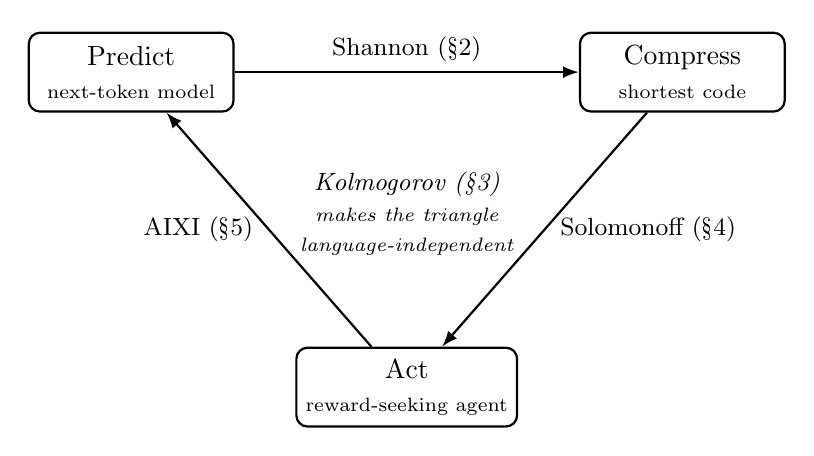
\begin{tikzpicture}[
  vertex/.style={draw, rounded corners, align=center, minimum width=2.6cm, minimum height=1cm, thick},
  edge/.style={-{Latex[length=2mm]}, thick}
]
  \node[vertex] (P) at (0,0) {Predict\\ \scriptsize next-token model};
  \node[vertex] (C) at (7,0) {Compress\\ \scriptsize shortest code};
  \node[vertex] (A) at (3.5,-4) {Act\\ \scriptsize reward-seeking agent};

  \draw[edge] (P) -- node[above, font=\small] {Shannon (\S2)} (C);
  \draw[edge] (C) -- node[right, font=\small, xshift=2pt] {Solomonoff (\S4)} (A);
  \draw[edge] (A) -- node[left, font=\small, xshift=-2pt] {AIXI (\S5)} (P);

  \node[font=\small\itshape, align=center] at (3.5,-1.8) {Kolmogorov (\S3)\\ \scriptsize makes the triangle\\ \scriptsize language-independent};
\end{tikzpicture}
\caption{The three-vertex picture. Each edge is a theorem that
translates one vertex into another. Kolmogorov complexity
(\S3) is the hub that makes the translation coordinate-free.}
\label{fig:triangle}
\end{figure}

\subsection*{Why this matters for decisions, not just for theory}

A decision-maker evaluating a foundation-model vendor faces a
simple but hard question: \emph{is the loss number on the vendor's
training dashboard a proxy for anything you care about?} If the
equivalence we are about to prove holds cleanly, the answer is yes:
every 0.1-bit improvement in held-out cross-entropy corresponds to
a measurable improvement in downstream capability, and the
conversion rate can be estimated. If the equivalence leaks --- and
we will show exactly where it does --- the answer is ``sometimes,
in these regimes, with these caveats.'' Either answer is
actionable; neither is available without the chain of theorems.

\begin{activity}[title={Activity A4 --- Falsification worksheet}]
Fill the table below before reading further. We will return to it
in \cref{sec:caveats} and see which of your rows survives.
\smallskip

\begin{tabular}{p{4.2cm}p{4.2cm}p{4.2cm}}
\toprule
\textbf{Equivalence claim} & \textbf{What would refute it} & \textbf{What is merely consistent} \\
\midrule
Lower bpc $\Rightarrow$ higher MMLU (same size). & & \\
Better zip ratio on a domain $\Rightarrow$ better agent on that domain. & & \\
A model that memorises (does not generalise) cannot compress held-out data well. & & \\
\bottomrule
\end{tabular}
\end{activity}

\paragraph{A caveat, promoted out of the footnotes.}
A \emph{perfect} next-token predictor would be an ideal learner.
Real next-token predictors are not perfect. The gap between them
and the ideal is exactly where this document's caveats live
(\cref{sec:caveats}); we state the thesis before we qualify it,
but the qualification is not optional. In particular: the
equivalence is between the \emph{training objective} and general
capability, not between any specific checkpoint and general
capability. A model can be a poor compressor of your domain while
the objective it was trained on remains the right objective. Keep
the distinction; a lot of vendor arguments blur it.

\medskip
\noindent\textbf{Formal statement of the thesis.}
The central technical claim of this note is that three operations
often treated as distinct --- predicting the next symbol in a
sequence, compressing that sequence into a shorter description, and
behaving intelligently in its presence --- are, under a precise set
of definitions, the \emph{same operation} viewed from three angles.
Shannon's source coding theorem \citep{shannon1948mathematical}
identifies prediction with compression; Kolmogorov complexity
\citep{kolmogorov1965three} makes the notion of ``shortest
description'' independent of the choice of description language;
Solomonoff's universal prior \citep{solomonoff1964formal} promotes
the Kolmogorov minimiser to a Bayesian predictor that converges to
any computable source; and Hutter's AIXI
\citep{hutter2005universal} upgrades that predictor into a
reward-seeking agent whose optimality can be stated as a theorem.
The chain is not an analogy. Every step in this note is a
definition, a lemma, or a theorem. The pedagogical payoff is that
one can then ask sharp questions about large language models ---
whether they count as compressors, whether better compression
entails more general capability, and where the equivalence breaks
--- without smuggling in metaphor.

% ========================= SECTION 2 (Shannon prelude) =========================
% =========================================================================

\section{Prelude: Shannon and the cost of surprise}
\label{sec:shannon-prelude}

\begin{intuition}
Information is the price you pay for being surprised, and you are
surprised in exact proportion to how unlikely an event was. Keep
three numbers in mind for the rest of this section:

\begin{itemize}[leftmargin=2em,itemsep=1pt]
  \item \textbf{Fair coin.} $p(\text{heads}) = \tfrac12$. One yes/no
    question settles it: $H = 1$ bit per flip.
  \item \textbf{Biased coin, 7/8 heads.} Most flips are boring;
    occasionally a tail surprises you. The average surprise works out
    to
    \[
      H = -\tfrac78\log_2\tfrac78 - \tfrac18\log_2\tfrac18
        \;\approx\; 0.169 + 0.375 \;=\; 0.544 \text{ bits per flip}.
    \]
    That is the ``about half a bit'' we promised --- now with the
    arithmetic to back it up.
  \item \textbf{A 1-in-1024 event.} $-\log_2(1/1024) = 10$ bits of
    ``wow.'' A 50/50 event carries one bit of ``huh.''
\end{itemize}

Two forecasters make this concrete. In Los Angeles, Ana says
``sunny'' nearly every day and is right nearly every day; her
distribution over \{sun, cloud, rain\} is roughly
$(0.85, 0.10, 0.05)$, so $H(\text{LA}) \approx 0.74$ bits per day.
In Zurich, B\"arbel faces \{sun, cloud, rain, snow, F\"{o}hn, fog\}
with a distribution closer to $(0.25, 0.30, 0.25, 0.07, 0.03, 0.10)$,
giving $H(\text{ZRH}) \approx 2.32$ bits per day. If the newspaper
pays each forecaster one cent per bit transmitted, B\"arbel earns
about three times what Ana does --- not because Zurich is colder,
but because Zurich is \emph{less predictable}. Shannon's
source-coding theorem (\cref{thm:source-coding}) says neither can do
better than her own entropy floor, no matter how clever her code.

\textbf{Why a decision-maker should care.} Every storage bill, every
bandwidth bill, every ``our model is more efficient'' vendor claim
bottoms out against an entropy floor. Printed English has entropy
between about $0.6$ and $1.3$ bits per character \citep[Ch.~6]{coverthomas2006};
if a vendor tells you they compress English text to $0.3$ bits per
character, they are either wrong, lying, or have discovered English
has lower entropy than anyone thought --- which would itself be news
on the scale of cold fusion. Entropy also sets the floor on
forecasting: no analyst, human or machine, can predict a genuinely
high-entropy process (next week's lottery numbers) better than
chance, no matter how much compute you throw at it. Knowing where
the entropy floor sits for \emph{your} data is the difference
between a reasonable AI budget and a fantasy one.
\end{intuition}

\subsection*{Formal setup}

Fix a finite \emph{alphabet} $\mathcal{A} = \{a_1, \dots, a_K\}$ and
let $X$ be a discrete random variable on $\mathcal{A}$ with
probability mass function $p(a) = \Pr[X = a]$. All logarithms are
base $2$ unless stated; values are measured in \emph{bits}. The
alphabet could be \{heads, tails\} for a coin, \{A, C, G, T\} for a
DNA base, the 256 possible bytes in a file, or the roughly $50{,}000$
sub-word tokens inside a modern language model.

\begin{definition}[Self-information and Shannon entropy]
\label{def:entropy}
The \textbf{self-information} (or \emph{surprisal}) of the outcome
$x \in \mathcal{A}$ under $p$ is
\begin{equation}
  I_p(x) \;=\; -\log_2 p(x),
  \label{eq:self-info}
\end{equation}
with the convention $0 \cdot \log_2 0 = 0$. The \textbf{Shannon
entropy} of $X$ is the expected self-information,
\begin{equation}
  H(X) \;=\; \mathbb{E}\bigl[I_p(X)\bigr]
       \;=\; -\sum_{k=1}^{K} p(a_k)\,\log_2 p(a_k).
  \label{eq:entropy}
\end{equation}
\end{definition}

\begin{aside}[title={Why the logarithm?}]
Three demands pin down $-\log_2 p$ up to the choice of base.
(i) A sure event ($p=1$) should carry zero surprise: $\log 1 = 0$.
(ii) Rarer events should carry more surprise: $-\log p$ is decreasing
in $p$. (iii) Independent surprises should \emph{add}: if $X$ and
$Y$ are independent, the surprise of seeing both is
$-\log(p_X p_Y) = -\log p_X - \log p_Y$. Only the logarithm turns
multiplication of probabilities into addition of surprise, which is
exactly what ``number of yes/no questions'' demands.
\end{aside}

\subsection*{Codes, trees, and Kraft}

A \textbf{code} for $\mathcal{A}$ is an injective map
$C : \mathcal{A} \to \{0,1\}^*$ assigning a binary string $C(a)$ to
each symbol. We write $\ell(a) = |C(a)|$ for the code length. $C$
is a \textbf{prefix code} (or \emph{instantaneous code}) if no
codeword $C(a_i)$ is a proper prefix of any other codeword $C(a_j)$.
The prefix property is what lets a receiver decode a stream of
codewords without delimiters: as soon as the bits read match a
codeword, that codeword is committed.

\begin{figure}[h]
\centering
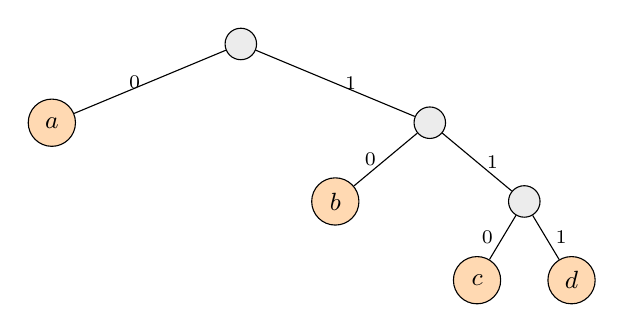
\begin{tikzpicture}[
  level distance=10mm,
  level 1/.style={sibling distance=48mm},
  level 2/.style={sibling distance=24mm},
  level 3/.style={sibling distance=12mm},
  every node/.style={font=\small},
  leaf/.style={draw, circle, fill=orange!30, inner sep=1pt, minimum size=6mm},
  inner/.style={draw, circle, fill=gray!15, inner sep=1pt, minimum size=4mm},
  edgelab/.style={font=\scriptsize, midway}
]
\node[inner] {}
  child {node[leaf] {$a$} edge from parent node[edgelab, left] {$0$}}
  child {node[inner] {}
    child {node[leaf] {$b$} edge from parent node[edgelab, left] {$0$}}
    child {node[inner] {}
      child {node[leaf] {$c$} edge from parent node[edgelab, left] {$0$}}
      child {node[leaf] {$d$} edge from parent node[edgelab, right] {$1$}}
      edge from parent node[edgelab, right] {$1$}
    }
    edge from parent node[edgelab, right] {$1$}
  };
\end{tikzpicture}
\caption{Prefix-code tree for the code $C(a)=0,\ C(b)=10,\
C(c)=110,\ C(d)=111$. Each leaf is a codeword; no codeword lies on
the path to another. The subtree rooted at depth $\ell$ covers a
$2^{-\ell}$ fraction of the infinite leaves, which is the content of
Kraft's inequality.}
\label{fig:prefix-tree}
\end{figure}

\begin{lemma}[Kraft's inequality]
\label{lem:kraft}
For any prefix code $C$ on $\mathcal{A}$ with lengths $\ell(a_k)$,
\begin{equation}
  \sum_{k=1}^{K} 2^{-\ell(a_k)} \;\le\; 1.
  \label{eq:kraft}
\end{equation}
Conversely, for any length assignment $\ell_1, \dots, \ell_K \in
\mathbb{N}$ satisfying~\eqref{eq:kraft} there exists a prefix code
with those lengths.
\end{lemma}

\begin{proof}[Proof sketch]
Identify each codeword with a leaf in the infinite binary tree
(\cref{fig:prefix-tree}). A prefix condition forbids any codeword
from lying on the path to another, so distinct codewords correspond
to \emph{disjoint} subtrees. The subtree rooted at a node of depth
$\ell$ contains a $2^{-\ell}$ fraction of the infinite leaves, and
disjointness of those fractions gives the bound. The converse is an
explicit construction: sort $\ell_k$ in increasing order and assign
the lexicographically smallest available length-$\ell_k$ string at
each step.
\end{proof}

\begin{example}[Entropy of a 4-symbol alphabet, revisited early]
\label{ex:h4}
Let $\mathcal{A} = \{a, b, c, d\}$ with $p(a) = \tfrac{1}{2}$,
$p(b) = \tfrac{1}{4}$, $p(c) = p(d) = \tfrac{1}{8}$. Then
\begin{align*}
  H(X) &= -\tfrac{1}{2}\log_2\tfrac{1}{2}
         - \tfrac{1}{4}\log_2\tfrac{1}{4}
         - 2\cdot\tfrac{1}{8}\log_2\tfrac{1}{8} \\
       &= \tfrac{1}{2}\cdot 1 + \tfrac{1}{4}\cdot 2 + \tfrac{1}{4}\cdot 3
        \;=\; \tfrac{7}{4} \text{ bits}.
\end{align*}
The prefix code $C(a) = 0,\ C(b) = 10,\ C(c) = 110,\ C(d) = 111$ of
\cref{fig:prefix-tree} achieves expected length
$L = \tfrac12\cdot 1 + \tfrac14\cdot 2 + \tfrac18\cdot 3 + \tfrac18\cdot 3
= \tfrac74$ bits exactly. Its lengths $(1,2,3,3)$ satisfy Kraft with
\emph{equality} and match $-\log_2 p(a_k)$ symbol by symbol. When
probabilities are negative powers of two, the Shannon floor is hit on
the nose.
\end{example}

\begin{activity}[title={Guess-the-next-flip bet game --- 10 minutes}]
\label{act:bet}
Pair students up. One student flips a coin biased 3/4 heads
(simulated by rolling a d4: 1--3 $=$ heads, 4 $=$ tails); the other
bets any fraction of a running 16-chip stake on the outcome. The
house rule: if you bet fraction $f$ on the outcome that actually
occurs and the true probability was $p$, your stake is multiplied by
$2f/(2p) = f/p$.\footnote{The Kelly-optimal fraction is $f=p$, which
multiplies the stake by $1$ on average; deviations lose in the long
run. Over many rounds the log-growth rate is
$\sum_x q(x)\log_2(f(x)/p(x))$, a KL divergence.}
Play ten rounds, then compute per round
\[
  \text{(avg. chips lost)} \;\approx\; D_{\mathrm{KL}}(p \,\|\, q)
  \;=\; \sum_x p(x)\log_2\tfrac{p(x)}{q(x)},
\]
where $q$ is the student's betting distribution. The class discovers
\emph{experimentally} that the only way not to bleed chips is to bet
$q = p$, and that their average loss equals the gap between the
cross-entropy they ``paid'' and Shannon's floor $H(p)$.
\textit{Leo:} a scoreboard he can compute round by round.
\textit{Yuki:} bits become chips.
\end{activity}

\subsection*{Gibbs' inequality: the wrong code pays a tax}

\begin{lemma}[Gibbs' inequality]
\label{lem:gibbs}
For any two probability mass functions $p, q$ on $\mathcal{A}$,
\begin{equation}
  -\sum_{k} p(a_k) \log_2 q(a_k)
    \;\ge\; -\sum_{k} p(a_k) \log_2 p(a_k),
  \label{eq:gibbs}
\end{equation}
with equality if and only if $p = q$.
\end{lemma}

\begin{aside}[title={A one-picture reason to believe $\ln x \le x - 1$}]
The curve $y = \ln x$ is concave; its tangent at $x = 1$ is the line
$y = x - 1$. A concave curve lies on or below any of its tangents,
so $\ln x \le x - 1$ everywhere, with equality exactly at $x = 1$.
Draw the two curves on the same axes once; you will never forget
this inequality again.
\end{aside}

\begin{proof}
Using $\ln x \le x - 1$ (with equality iff $x = 1$) and
$\log_2 x = \ln x / \ln 2$,
\[
  \sum_k p(a_k) \log_2 \frac{q(a_k)}{p(a_k)}
  \;\le\; \frac{1}{\ln 2}\sum_k p(a_k)\!\left(\frac{q(a_k)}{p(a_k)} - 1\right)
  \;=\; \frac{1}{\ln 2}\Bigl(\sum_k q(a_k) - 1\Bigr) \;\le\; 0,
\]
because $\sum_k q(a_k) \le 1$. Rearranging gives~\eqref{eq:gibbs};
the equality conditions of $\ln x \le x - 1$ and $\sum q = 1$
together force $p = q$.
\end{proof}

\begin{intuition}[title={What Gibbs really says}]
If the world is distributed as $p$ but you design a code as if the
world were distributed as $q$, you pay $-\sum p\log q$ bits on
average instead of $-\sum p\log p$. The difference,
\[
  D_{\mathrm{KL}}(p \,\|\, q)
    \;=\; \sum_k p(a_k) \log_2 \tfrac{p(a_k)}{q(a_k)},
\]
is the \emph{tax} the world levies on your wrong model. It is
non-negative, zero only when $q=p$, and we will meet it again under
the name ``cross-entropy loss'' whenever a neural network is being
trained.
\end{intuition}

\subsection*{Shannon's source-coding theorem}

\begin{theorem}[Shannon source-coding inequality]
\label{thm:source-coding}
Let $C$ be any uniquely decodable (in particular, any prefix) code
for $\mathcal{A}$ and let $L = \mathbb{E}[\ell(X)] =
\sum_k p(a_k)\ell(a_k)$ be its expected code length. Then
\begin{equation}
  L \;\ge\; H(X).
  \label{eq:source-coding}
\end{equation}
Moreover, there exists a prefix code (e.g.\ the Shannon--Fano code
with $\ell(a_k) = \lceil -\log_2 p(a_k)\rceil$) such that
\begin{equation}
  L \;<\; H(X) + 1.
  \label{eq:source-coding-achiev}
\end{equation}
\end{theorem}

\begin{proof}[Proof sketch]
Let $q(a_k) = 2^{-\ell(a_k)} / Z$, where
$Z = \sum_k 2^{-\ell(a_k)} \le 1$ by \cref{lem:kraft}; so $q$ is a
bona fide probability vector. Read $q$ as the \emph{implicit model}
your code $C$ is betting on: it assigns probability $q(a_k)$ to
symbol $a_k$ because it spent $\ell(a_k)$ bits describing it. By
\cref{lem:gibbs}, the cross-entropy $-\sum_k p(a_k) \log_2 q(a_k)
\ge H(X)$, i.e.\ the wrong model pays a tax. Because
$-\log_2 q(a_k) = \ell(a_k) + \log_2 Z \le \ell(a_k)$ (since $Z \le
1$ makes $\log_2 Z \le 0$), we get $L \ge -\sum_k p(a_k)\log_2
q(a_k) \ge H(X)$. For~\eqref{eq:source-coding-achiev}, the lengths
$\lceil -\log_2 p(a_k)\rceil$ satisfy Kraft~\eqref{eq:kraft}, and
each ceiling adds at most $1$ to the expected length. See
\citet[Ch.~5]{coverthomas2006} for the full treatment.
\end{proof}

\begin{aside}[title={The slogan, properly qualified}]
``Every code is a probability model and every probability model is a
code.'' Precisely: a prefix code with lengths $\ell(a_k)$ implicitly
asserts the distribution $q(a_k) \propto 2^{-\ell(a_k)}$; a
distribution $q$ suggests lengths $\lceil -\log_2 q(a_k)\rceil$.
When we train a language model to minimise cross-entropy loss, we
are literally minimising the expected code length under Shannon's
theorem. This is the hinge that the rest of these notes turns on.
\end{aside}

\subsection*{More worked examples}

\begin{example}[Back to the 4-symbol alphabet, with a wrong model]
\label{ex:h4-wrong}
Keep $p = (\tfrac12, \tfrac14, \tfrac18, \tfrac18)$ but design a code
as if the distribution were uniform, $q = (\tfrac14, \tfrac14,
\tfrac14, \tfrac14)$, giving two bits per symbol to every letter.
Then $L = 2$ bits, the cross-entropy is $-\sum p \log_2 q = 2$ bits,
and the KL tax is $D_{\mathrm{KL}}(p\|q) = 2 - \tfrac74 = \tfrac14$
bit per symbol. Over a million symbols, betting on uniform instead
of $p$ costs you $250{,}000$ bits --- about $31$ kilobytes of
wasted bandwidth.
\end{example}

\begin{example}[Biased coin, bit by bit]
\label{ex:biased-coin}
The $7/8$-heads coin has $H \approx 0.544$ bits. You cannot encode
one flip in fewer than one bit, of course --- codewords are
integer-length. But if you block flips in groups of $10$, the
block alphabet has $2^{10} = 1024$ outcomes and the block entropy
is $10\cdot 0.544 = 5.44$ bits, which Shannon--Fano reaches to
within one bit. Long-run bandwidth drops from $10$ bits per block
(naive) to about $6$ bits per block. This is why every real
compressor (gzip, arithmetic coding, LLM tokenisers) works on
blocks or streams, not symbol-by-symbol.
\end{example}

\begin{activity}[title={Entropy of your phone lock-screen --- 5 minutes}]
\label{act:pin}
On scrap paper, write down (1) the length $n$ of your phone PIN or
pattern, (2) whether it contains a birthday (your own, a partner's,
a child's), and (3) whether it repeats a digit. Using the prior
\[
  p(\text{PIN}) \approx
  \begin{cases}
    3\times 10^{-3} & \text{if birthday-shaped}, \\
    10^{-n}          & \text{otherwise},
  \end{cases}
\]
compute $-\log_2 p$ in bits. Compare to the entropy of a uniformly
random $n$-digit PIN, $n \log_2 10 \approx 3.32 n$ bits. The typical
result in a classroom is that ``birthday'' PINs land near $8$--$9$
bits while a truly random 6-digit PIN is near $20$ bits. That
$\sim 11$-bit gap is the factor-of-$2000$ advantage a thief enjoys
against the average human.
\textit{Yuki:} personally concrete. \textit{Leo:} ends in a number.
\end{activity}

\begin{activity}[title={Huffman-code-by-hand worksheet --- 15 minutes}]
\label{act:huffman}
Given probabilities $p = (0.40, 0.20, 0.15, 0.15, 0.10)$ over
symbols $\{A,B,C,D,E\}$:
\begin{enumerate}[leftmargin=2em,itemsep=1pt]
  \item Sort and repeatedly merge the two lowest-probability symbols
    into a meta-symbol whose probability is their sum. Record each
    merge as a parent node.
  \item After four merges you have a single root. Label each left
    edge $0$ and each right edge $1$; read each leaf's codeword
    from the root.
  \item Compute $L = \sum p(a_k) \ell(a_k)$ and compare to
    $H(X) = -\sum p \log_2 p \approx 2.15$ bits. The Huffman code
    achieves $L = 2.20$ bits, within $0.05$ of entropy.
  \item \textit{Stretch:} change $p(A)$ from $0.40$ to $0.95$ and
    redo. Watch the code for $A$ collapse to a single bit while the
    others grow. This is the shape of \emph{adaptive} compression.
\end{enumerate}
\textit{Leo:} pencil-and-paper payoff. \textit{Yuki:} the tree
becomes a physical drawing.
\end{activity}

\begin{activity}[title={Six lines of Python --- take home}]
\label{act:python}
Paste this into any Python 3 prompt:
\begin{verbatim}
from collections import Counter
from math import log2
def H(s):
    n = len(s)
    return -sum((c/n)*log2(c/n) for c in Counter(s).values())
print(H("to be or not to be that is the question"))
\end{verbatim}
Run it on (a) the first paragraph of a novel in your native
language, (b) the same paragraph translated to English, and (c) a
200-character string of your own keystrokes. You will typically see
$H \approx 4.2$ bits per character on natural-language prose and
$H \approx 3.0$ on keystrokes from a human who has a strong
hand-preference. The true entropy of English is lower
(${\sim}1$ bit/char) because this snippet ignores correlations
between neighbouring characters --- which is exactly the gap a
language model closes.
\textit{Leo:} code he can execute. \textit{Yuki:} numbers for two
inputs he already cares about.
\end{activity}

\begin{aside}[title={Forward pointer}]
We will re-encounter cross-entropy in \cref{def:entropy}'s shadow
every time a neural network is trained; the KL tax will reappear as
the ``surprise'' of a held-out document under a language model; and
the source-coding theorem will become the statement that
\emph{prediction is compression} in the very next section.
\end{aside}

% ========================= SECTION 3 (Prediction = Compression) =========================


\section{Prediction \texorpdfstring{$\Leftrightarrow$}{<=>} Compression
         (Shannon's half of the bridge)}
\label{sec:pred-comp}

\begin{intuition}
A predictor that assigns probabilities to the next word is, mechanically,
a compressor; its error rate and its compression rate are the same
number wearing different clothes (see \cref{thm:ce-code} and
\cref{cor:ppl}).

\medskip
\textbf{The two-consultants analogy (postage version).}  Two
consultants write up the same quarter.  Both are earnest.  The one
who understands your business writes a one-pager: \emph{revenue up
$4\%$, driven by Zurich, offset by FX.}  The one whose mental model
is slightly off writes ten pages of hedging --- because every
surprise in the data costs her extra sentences.  Both describe
reality perfectly; only one \emph{compresses} it.

Think of it as postage.  The true entropy $H(p)$ is the postage a
perfectly-informed sender pays.  Cross-entropy $H(p,q)$ is the
postage you actually pay when your delivery model is $q$ but the
world is $p$.  The difference, $H(p,q) - H(p)$, is the
\textbf{surcharge for being wrong}, and information theory has a
name for it: the Kullback--Leibler divergence $D_{\mathrm{KL}}(p\|q)$.

\medskip
\textbf{A concrete, addable number.}  Suppose tomorrow's stock move
is \emph{up} with probability $0.9$ and \emph{down} with probability
$0.1$.  The true entropy is
\[
 H(p) = -0.9\log_2 0.9 - 0.1\log_2 0.1 \approx 0.469 \text{ bits/day.}
\]
If your model believes the market is $50/50$, you spend exactly $1$
bit per day describing it.  The surcharge is
$1 - 0.469 \approx 0.531$ bits per day.  Over a million days (or
tokens) that is
\[
  0.531 \times 10^{6} \approx 5.3 \times 10^{5} \text{ extra bits,}
\]
roughly $66$ kilobytes of \emph{pure hedging}, paid because the model
was wrong about the coin.

\medskip
\textbf{Perplexity in one sentence.}  LLM papers report ``perplexity
$8$'' or ``$2.1$ bits per token.''  These are the same number:
$\log_2 8 = 3$ bits per token; $\log_2(\mathrm{PPL}) =$ bits per
token $=$ cross-entropy (\cref{cor:ppl}).  \emph{Perplexity $8$
means the model behaves as if at each word it were choosing
uniformly among $8$ plausible options.}  Lower is better.

\medskip
\textbf{Why a decision-maker should care.}  The training objective
of every major LLM \emph{is} cross-entropy on text.  When a vendor
says ``our model scored $0.1$ lower cross-entropy,'' they are saying
``our model compresses the world $0.1$ bits better per word,'' which
over trillions of words is a lot of real modelling skill.  Two
models with identical cross-entropy are, at the level Shannon cares
about, the same model.  This gives you a vendor-agnostic yardstick
--- and a cheap test for benchmark theatre: if a new model does not
improve cross-entropy but wins on a specific test, ask whether the
test was in the training set.
\end{intuition}


% ---------------------------------------------------------------------
\subsection*{From analogy to definition}
% ---------------------------------------------------------------------

Before the formalism, a one-line vocabulary bridge: a \emph{prefix
code} is a dictionary that assigns each symbol a unique bit-string
such that no codeword is a prefix of another --- so a decoder can
unambiguously split a stream back into symbols.  A \emph{good} model
$q$ assigns high probability to the symbols that actually occur;
the corresponding code is short exactly when $q$ is accurate.  Keep
that picture as you read the definitions.

Sequence models predict \emph{conditionally}.  Fix a stochastic
process $(X_t)_{t \ge 1}$ on $\mathcal{A}$ and write
$X_{<t} = (X_1, \dots, X_{t-1})$ with $X_{<1} = \emptyset$.

\begin{definition}[Cross-entropy and conditional cross-entropy]
\label{def:cross-ent}
Let $p$ be the true distribution of $(X_1, \dots, X_T)$ and let $q$
be a model distribution that factors autoregressively,
$q(x_{1:T}) = \prod_{t=1}^{T} q(x_t \mid x_{<t})$.  The
\textbf{cross-entropy} of $q$ against $p$ at position $t$ is
\begin{equation}
  H_t(p, q)
  \;=\; \mathbb{E}_{x_{<t}\sim p}\!\left[
    -\sum_{a\in\mathcal{A}} p(a \mid x_{<t})\,\log_2 q(a \mid x_{<t})
  \right],
  \label{eq:cross-ent}
\end{equation}
and the \textbf{average cross-entropy per token} is
$\overline{H}(p,q) = \tfrac{1}{T}\sum_{t=1}^{T} H_t(p,q)$.
\end{definition}

\noindent
\emph{Read-aloud translation.}  ``If the world draws symbols from
$p$ but you describe them with $q$, equation~\eqref{eq:cross-ent} is
the \emph{average number of bits} it will cost per symbol.''

\begin{theorem}[Cross-entropy equals expected code length]
\label{thm:ce-code}
Fix $T$ and a model $q$.  Any prefix code that uses
$\ell(x_t \mid x_{<t}) = \lceil -\log_2 q(x_t \mid x_{<t})\rceil$
bits to encode $x_t$ given $x_{<t}$ satisfies
\begin{equation}
  \mathbb{E}_{x_{1:T}\sim p}\!\left[\tfrac{1}{T}\!\sum_{t=1}^{T}\ell(x_t \mid x_{<t})\right]
  \;=\; \overline{H}(p, q) + O(1/T),
  \label{eq:ce-length}
\end{equation}
and arithmetic coding attains~\eqref{eq:ce-length} with $O(1/T)$
overhead.  Moreover,
\begin{equation}
  \overline{H}(p, q)
  \;=\; \overline{H}(p) + \overline{D}_{\mathrm{KL}}(p \,\|\, q),
  \label{eq:ce-kl}
\end{equation}
where $\overline{H}(p) = \tfrac{1}{T}\sum_t H(X_t \mid X_{<t})$ is
the true conditional entropy rate and
$\overline{D}_{\mathrm{KL}}(p\|q) \ge 0$ is the average conditional
Kullback--Leibler divergence.
\end{theorem}

\begin{proof}[Proof of~\eqref{eq:ce-kl}]
For each $t$ and each history $x_{<t}$,
\[
  -\sum_{a} p(a\!\mid\! x_{<t})\log_2 q(a\!\mid\! x_{<t})
  \;=\;
  -\sum_{a} p(a\!\mid\! x_{<t})\log_2 p(a\!\mid\! x_{<t})
  + \sum_a p(a\!\mid\! x_{<t})\log_2\frac{p(a\!\mid\! x_{<t})}{q(a\!\mid\! x_{<t})}.
\]
The first term on the right is $H(X_t \mid X_{<t} = x_{<t})$; the
second is
$D_{\mathrm{KL}}(p(\cdot\mid x_{<t})\,\|\,q(\cdot\mid x_{<t}))$.
Taking expectation over $x_{<t} \sim p$ and averaging over $t$
yields~\eqref{eq:ce-kl}.  Non-negativity of the KL term is exactly
\textbf{Gibbs' inequality} (\cref{lem:gibbs}): for any two
distributions $p, q$ on the same support,
$-\sum_a p(a)\log q(a) \ge -\sum_a p(a)\log p(a)$, with equality iff
$p = q$.  Statement~\eqref{eq:ce-length} follows by plugging
$\ell = \lceil -\log_2 q\rceil$ into \cref{thm:source-coding} on
each conditional distribution and absorbing the at-most-$1$-bit
rounding into the $O(1/T)$ overhead; arithmetic coding eliminates
even the integer ceilings up to a constant
\citep[Ch.~5]{coverthomas2006}.
\end{proof}

\begin{corollary}[Perplexity vs.\ bits per token]
\label{cor:ppl}
The \textbf{perplexity} of $q$ on $p$ is
$\mathrm{PPL}(q) = 2^{\overline{H}(p,q)}$, so
\begin{equation}
  \log_2 \mathrm{PPL}(q) \;=\; \overline{H}(p,q)
  \;=\; \text{(bits per token used by arithmetic coding with model }q\text{)}.
  \label{eq:ppl-bpt}
\end{equation}
In words: \emph{perplexity is the effective branching factor; bits
per token is its $\log_2$; they are two dials on the same gauge.}
\end{corollary}

\Cref{thm:ce-code} is the entire Shannon side of the bridge:
\emph{minimising the cross-entropy training objective is literally
minimising the expected compressed length}.  A next-token predictor
with cross-entropy $\overline{H}(p,q)$ bits per symbol corresponds,
via arithmetic coding, to a compressor that uses
$\overline{H}(p,q)$ bits per symbol.  Better predictions
$\Leftrightarrow$ shorter codes.


% ---------------------------------------------------------------------
\subsection*{Concrete handles}
% ---------------------------------------------------------------------

\begin{activity}[title={Activity 3.A --- Compress your own message (paper, 10 min)}]
\label{act:compress-paper}
You are given an alphabet $\mathcal{A} = \{A, B, C, D\}$ with true
distribution
\[
 p(A) = \tfrac{1}{2}, \quad p(B) = \tfrac{1}{4}, \quad
 p(C) = \tfrac{1}{8}, \quad p(D) = \tfrac{1}{8}.
\]
\textbf{Tasks.}
\begin{enumerate}[leftmargin=*, itemsep=2pt]
  \item Compute $H(p)$ in bits.  (Answer: $1.75$ bits/symbol.)
  \item Design a prefix code.  Hint: assign the shortest codeword to
        the most common symbol.  One valid choice: $A\!\mapsto\!0$,
        $B\!\mapsto\!10$, $C\!\mapsto\!110$, $D\!\mapsto\!111$.
  \item Compute expected code length
        $\mathbb{E}[\ell] = \sum_a p(a)\ell(a)$.  Compare to $H(p)$.
        (You should hit the entropy exactly --- this code is
        \emph{optimal}.)
  \item Now pretend your model was $q(A)=q(B)=q(C)=q(D)=\tfrac{1}{4}$
        (uniform).  The natural code is $2$ bits per symbol.
        Expected length under \emph{true} $p$ is still $2$.  The
        surcharge $2 - 1.75 = 0.25$ bits/symbol is
        $D_{\mathrm{KL}}(p\|q)$.  Verify this by computing
        $\sum_a p(a)\log_2\frac{p(a)}{q(a)}$.
\end{enumerate}
\emph{This is \cref{thm:ce-code} on one page of paper.}
\end{activity}

\begin{activity}[title={Activity 3.B --- Role-play: the two consultants (3 min)}]
\label{act:consultants}
Pair up.  Partner $X$ reads the \emph{matched} consultant's lines;
partner $Y$ reads the \emph{mismatched} consultant's lines.  Both
describe the same quarter.

\textbf{Matched consultant ($q = p$):}
\begin{enumerate}[leftmargin=*, itemsep=0pt, label=(M\arabic*)]
  \item ``Revenue up $4\%$.''
  \item ``Zurich drove growth.''
  \item ``FX was a drag.''
\end{enumerate}

\textbf{Mismatched consultant ($q \ne p$):}
\begin{enumerate}[leftmargin=*, itemsep=0pt, label=(W\arabic*)]
  \item ``Revenue is up, but only if we exclude these adjustments,
        and those adjustments, and also the following footnote \dots''
  \item ``Several offices contributed; Zurich was one of many; let me
        also describe Geneva, Basel, and Lugano \dots''
  \item ``FX might have helped or hurt; depending on the basket I
        reconstruct from scratch \dots''
\end{enumerate}

\textbf{Debrief.}  The mismatched consultant is not lying; she is
\emph{paying the KL surcharge} in sentences.  Name the cost: each
extra word is a bit.
\end{activity}

\begin{activity}[title={Activity 3.C --- Per-token cross-entropy in 6 lines of Python}]
\label{act:python-sec3}
Run this mentally or on a laptop.  Two toy models assign
probabilities to the three tokens of ``the cat sat.''
\begin{lstlisting}[language=Python]
import math
p_good = [0.5, 0.4, 0.3]    # model A's P(token_t | history)
p_bad  = [0.1, 0.05, 0.02]  # model B's P(token_t | history)
ce = lambda probs: -sum(math.log2(x) for x in probs) / len(probs)
print("A:", round(ce(p_good), 3), "bits/token")   # 1.442
print("B:", round(ce(p_bad),  3), "bits/token")   # 4.738
\end{lstlisting}
\emph{Interpretation.}  Model A spends $\approx 1.44$ bits per
token; Model B spends $\approx 4.74$.  On a million-token corpus,
Model B wastes $\approx (4.74-1.44)\times 10^{6} / 8 \approx 413$~KB
\emph{per sentence's worth of surprise} --- a vivid way to see why
vendors chase tenths of a bit.
\end{activity}

\begin{activity}[title={Activity 3.D --- Perplexity $\to$ bytes saved (numerical, 5 min)}]
\label{act:bytes}
Vendor $V_1$ reports perplexity $8$; vendor $V_2$ reports perplexity
$4.29$.  A $1$M-token corpus is about to be archived.
\begin{enumerate}[leftmargin=*, itemsep=2pt]
  \item $V_1$: $\log_2 8 = 3.0$ bits/token.
  \item $V_2$: $\log_2 4.29 \approx 2.1$ bits/token.
  \item Difference: $0.9$ bits/token.
  \item Over $10^{6}$ tokens: $9.0 \times 10^{5}$ bits $= 112{,}500$
        bytes $\approx 110$ KB \emph{saved} by choosing $V_2$.
  \item Over a trillion tokens ($10^{12}$): $\approx 110$ GB saved.
\end{enumerate}
\emph{Moral.}  Tiny-looking cross-entropy gaps are enormous at
corpus scale.  This is why frontier labs fight over the third
decimal.
\end{activity}


% --- TikZ bar chart: per-token surprise for "the cat sat" ---
\begin{figure}[h]
\centering
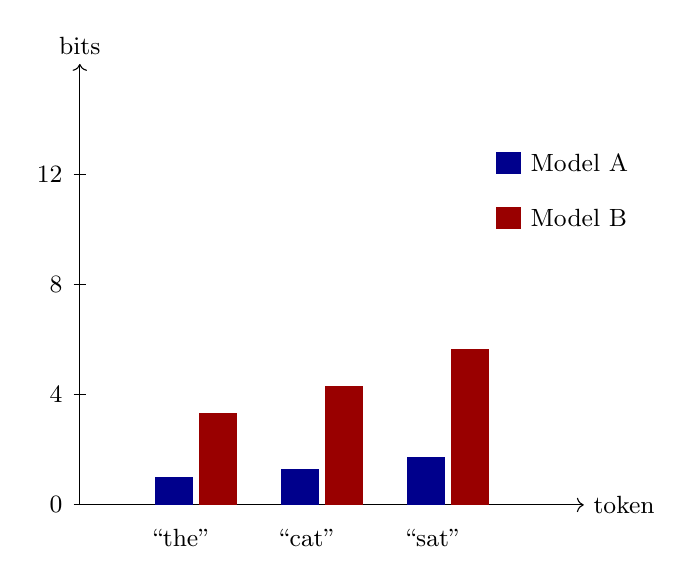
\begin{tikzpicture}[x=1.6cm, y=0.35cm]
  % axes
  \draw[->] (0,0) -- (4,0) node[right] {\small token};
  \draw[->] (0,0) -- (0,16) node[above] {\small bits};
  \foreach \y in {0,4,8,12} \draw (-0.05,\y) -- (0.05,\y) node[left,xshift=-5pt] {\small \y};
  % Model A bars (good): -log2(0.5, 0.4, 0.3) = 1.00, 1.32, 1.74
  \fill[blue!55!black] (0.6,0)  rectangle (0.9,1.00);
  \fill[blue!55!black] (1.6,0)  rectangle (1.9,1.32);
  \fill[blue!55!black] (2.6,0)  rectangle (2.9,1.74);
  % Model B bars (bad): -log2(0.1, 0.05, 0.02) = 3.32, 4.32, 5.64
  \fill[red!60!black]  (0.95,0) rectangle (1.25,3.32);
  \fill[red!60!black]  (1.95,0) rectangle (2.25,4.32);
  \fill[red!60!black]  (2.95,0) rectangle (3.25,5.64);
  % labels
  \node at (0.8,-1.2) {\small ``the''};
  \node at (1.8,-1.2) {\small ``cat''};
  \node at (2.8,-1.2) {\small ``sat''};
  % legend
  \fill[blue!55!black] (3.3,12) rectangle (3.5,12.8);
  \node[right] at (3.5,12.4) {\small Model A};
  \fill[red!60!black]  (3.3,10) rectangle (3.5,10.8);
  \node[right] at (3.5,10.4) {\small Model B};
\end{tikzpicture}
\caption{Per-token surprise $-\log_2 q(x_t\mid x_{<t})$ for the
sentence ``the cat sat'' under two toy models.  The total height is
the cross-entropy times $T$; the area difference is the KL
surcharge.  (\cref{act:python-sec3})}
\label{fig:surprise-bars}
\end{figure}


\begin{decisionbox}
\textbf{Three questions to ask an LLM vendor.}
\begin{enumerate}[leftmargin=*, itemsep=2pt]
  \item \emph{What is your held-out cross-entropy (or equivalently,
        perplexity) on a corpus we supply?}  This is the only
        vendor-agnostic compression score.
  \item \emph{Was the benchmark corpus demonstrably outside the
        training set?}  If not, the number is theatre.
  \item \emph{How much does a $0.1$-bit-per-token improvement cost in
        compute, and what does it buy at our deployment scale?}
        Use \cref{act:bytes} to translate bits into storage,
        bandwidth, or inference tokens.
\end{enumerate}
\end{decisionbox}

A worked numerical example separating the matched and mismatched
models on a $3$-token sequence is given in \cref{app:ce-worked};
\cref{act:python-sec3,act:bytes} above are the in-class shortcuts to the
same computation.

% =========================================================================

% ========================= SECTION 4 (Kolmogorov) =========================
\section{Kolmogorov complexity}
\label{sec:kolmogorov}

\begin{intuition}
\textbf{One-line answer.}  The Kolmogorov complexity $K(x)$ of an
object $x$ is the length, in bits, of the shortest computer program
that prints $x$ and stops (\cref{def:kolmogorov}).  It is the
vendor-independent floor on how far $x$ can ever be compressed.

\textbf{Twin USB sticks.}  Imagine two 8\,GB USB sticks on your desk.
One is full of family JPGs; the other is full of bytes drawn from
\texttt{/dev/urandom}.  Both weigh the same; both read the same number
of bits off the bus.  Zip the first and you get roughly
$6$--$7\,\text{GB}$; zip the second and you get back almost exactly
$8\,\text{GB}$ --- sometimes \emph{larger}, once zip's header is added.
The difference is not in the hardware.  It is a property of the
\emph{contents}: the photos have structure a short program can
exploit, the random bytes do not.  Kolmogorov complexity is the
mathematical name for that difference.

\textbf{The recipe-over-the-phone picture.}  You are a chef.  A
colleague in another city must reproduce your dish exactly.  You
dictate the shortest instructions that do the job.  ``Boil water''
takes two words.  A souffl\'e takes a page.  A pattern of $10{,}000$
genuinely random sprinkles on a cake has no shorter description than
itself: you read out every position.  Such an object is
\emph{Kolmogorov random}; it has no exploitable structure.  Everything
else --- the digits of $\pi$, the works of Shakespeare, your customer
database --- has a recipe shorter than the raw data.

\textbf{A tiny worked example.}  The string \texttt{01010101\ldots} (a
million characters long) has an $\approx 30$-character recipe:
\texttt{print "01" 500000 times}.  A million genuine coin flips has no
such shortcut; its recipe is, to within a small constant, a million
characters.  Same disk size, wildly different Kolmogorov complexity.
\emph{Complexity measures structure, not size.}

\textbf{Invariance and uncomputability, previewed.}  Two different
programming languages disagree about the length of a recipe by at most
the size of a translator between them (\cref{thm:invariance}).  So
$K(x)$ is a property of the object, not your toolkit.  But no
algorithm, given $x$, can hand you its shortest program
(\cref{thm:uncomputable}); if one existed, it would decide the halting
problem.  $K(x)$ is a perfectly well-defined number that you can bound
from above --- by running zip, by training a model --- but never
compute exactly.

\textbf{Why a decision-maker should care.}  Your company's data has a
\emph{true}, vendor-independent information content.  No one can quote
it to you exactly; anyone who claims to has sold you the Brooklyn
Bridge.  But every real compressor --- zip, JPEG, your LLM --- gives
you an upper bound, and upper bounds are enough to tell snake oil from
signal.
\end{intuition}

\begin{intuition}[title={The compression sniff test}]
If a vendor claims to losslessly compress genuinely random or properly
encrypted data, they are selling snake oil --- Shannon closed that
door in 1948.  A truly random source has entropy equal to its raw
bit-length; no code can do better on average
(\cref{thm:source-coding}).  ``We compress encrypted traffic by
40\,\%'' is either marketing about a non-random \emph{side channel}
(timestamps, packet sizes, TLS record framing) --- which may be
legitimate --- or a claim that should not appear in a contract you
sign.  Activity~\ref{act:bingo} gives you a bingo card for the next
vendor demo.
\end{intuition}

\begin{activity}[title={Activity 1 --- Shortest-recipe game}]
\label{act:recipe}
\textbf{Setup (10 minutes, pairs).}  Each pair receives the four
strings below.  Write, in the pseudocode of your choice, the shortest
program you can that prints each exactly.  Score: total characters
summed across the four programs.  Lowest score wins.

\begin{enumerate}[label=(\alph*),leftmargin=*]
  \item \texttt{01} repeated $500$ times (total length $1000$).
  \item The first $100$ decimal digits of $\pi$.
  \item The filename \texttt{IMG\_0423.JPG}.
  \item $100$ bytes freshly drawn from \texttt{/dev/urandom},
        printed as a $200$-character hex string (distributed on paper).
\end{enumerate}

\textbf{Debrief.}  Strings (a), (b), (c) collapse to tiny programs: a
loop, a formula, and a literal constant shorter than the output.
String (d) does not collapse: the shortest program anyone in the room
produces is essentially \texttt{print "<the 200 hex chars>"}.  You
have just re-derived, by hand, the distinction between
Kolmogorov-compressible and Kolmogorov-random objects.
\end{activity}

Shannon's framework is probabilistic: entropy is a property of a
distribution, not of an individual string.  Kolmogorov's move
\citep{kolmogorov1965three} was to attach a complexity measure to a
\emph{single} object by asking for the length of its shortest
description in a fixed universal language.

Fix once and for all a \textbf{universal Turing machine} $U$ --- a
machine that, given as input a description $\langle M, w\rangle$ of
any Turing machine $M$ and input $w$, simulates $M$ on $w$.

\begin{definition}[Kolmogorov complexity]
\label{def:kolmogorov}
The \textbf{Kolmogorov complexity} of a finite binary string
$x \in \{0,1\}^*$, relative to $U$, is
\begin{equation}
  K_U(x)
  \;=\; \min\bigl\{\, |\pi| \,:\, \pi \in \{0,1\}^*,\ U(\pi) = x \,\bigr\},
  \label{eq:kolmogorov}
\end{equation}
where $|\pi|$ is the bit-length of the program $\pi$ and $U(\pi) = x$
means $U$ on input $\pi$ halts with output $x$.
\end{definition}

\begin{activity}[title={Activity 2 --- The gzip-vs-$K$ scoreboard}]
\label{act:scoreboard}
\textbf{Setup (5 minutes, demo or take-home).}  For each of the four
strings from Activity~\ref{act:recipe}, measure three numbers:

\begin{enumerate}[label=(\roman*),leftmargin=*]
  \item \textbf{Raw size} --- the bit-length of the string itself.
  \item \textbf{\texttt{gzip -9} size} --- bit-length of the
        compressed file (subtract the $\sim\!80$-bit gzip header for
        tiny inputs, or just note it).
  \item \textbf{Shortest-recipe bound} --- the bit-length of the
        winning program from Activity~\ref{act:recipe}, converted to
        bits at $8$\,bit/character.
\end{enumerate}

Plot the three as a bar chart per string.  You will see: for (a)--(c)
the recipe bound sits far below gzip; for (d) all three bars are
essentially the same height.  The ``recipe bound'' is itself only an
upper bound on $K(x)$ --- the true $K(x)$ is uncomputable
(\cref{thm:uncomputable}) --- but seeing gzip dominated by a
one-line Python program is the fastest way to feel in your bones that
$K$ lives far below any off-the-shelf compressor.
\end{activity}

\begin{theorem}[Invariance theorem]
\label{thm:invariance}
If $U_1$ and $U_2$ are two universal Turing machines, then there
exists a constant $c_{U_1,U_2}$\footnote{The constant $c_{U_1,U_2}$
is finite and does not grow with $|x|$.  Concretely: the smallest
self-contained CPython interpreter in C is a few hundred kilobytes of
source, and a minimal C compiler written in Python is comparable; so
for the pair (Python, C), $c_{U_1,U_2}$ is on the order of
$10^6$--$10^7$ bits.  For a megabyte-scale corpus ($\sim\!10^7$ bits)
this is already a non-trivial fraction; for a one-gigabyte ERP export
($\sim\!10^{10}$ bits) it is numerically negligible, and
``machine-independent up to an additive constant'' is a property you
can plan around.  For objects \emph{smaller} than the constant --- a
one-sentence log entry, a password --- it is not, and quoting ``the''
Kolmogorov complexity of such an object is meaningless without fixing
$U$.}, depending on $U_1$ and $U_2$ but not on $x$, such that
\begin{equation}
  \bigl| K_{U_1}(x) - K_{U_2}(x) \bigr| \;\le\; c_{U_1,U_2}
  \quad \text{for every } x \in \{0,1\}^*.
  \label{eq:invariance}
\end{equation}
\end{theorem}

\begin{proof}[Proof sketch]
Because $U_1$ is universal, there is a fixed-length binary program
$s_{2\to 1}$ --- an interpreter for $U_2$ written for $U_1$ --- that,
when prepended to any $U_2$-program $\pi$, causes $U_1$ to simulate
$U_2(\pi)$.  Thus every $U_2$-program $\pi$ of length $|\pi|$ yields a
$U_1$-program of length $|s_{2\to 1}| + |\pi|$ with the same output,
giving $K_{U_1}(x) \le K_{U_2}(x) + |s_{2\to 1}|$.  Symmetrically with
$s_{1\to 2}$.  Taking $c_{U_1,U_2} = \max(|s_{1\to 2}|, |s_{2\to 1}|)$
gives~\eqref{eq:invariance}.
\end{proof}

By convention we henceforth write $K(x)$ and treat the universal
simulator as the additive constant.

\begin{intuition}[title={The Berry paradox, dramatised}]
Consider the English phrase
\begin{quote}
``the smallest positive integer not nameable in fewer than twenty
English words.''
\end{quote}
That phrase contains nineteen words.  So if the integer it picks out
exists, we have just named it in nineteen words, contradicting the
very property we used to pick it.  The paradox is resolved by noting
that ``nameable in English'' is too slippery to be a mathematical
predicate.  But if we replace ``nameable in English'' with ``printed
by a program of length $\le m$'', the slipperiness vanishes --- and
the same self-referential trick becomes a clean proof that $K$ cannot
be computed.  That is the content of \cref{thm:uncomputable}.
\end{intuition}

\begin{theorem}[Uncomputability of $K$]
\label{thm:uncomputable}
There is no total computable function $f : \{0,1\}^* \to \mathbb{N}$
such that $f(x) = K(x)$ for all $x$.
\end{theorem}

\begin{proof}[Proof (Berry-paradox style)]
Suppose for contradiction such an $f$ exists.  Define the program
$P_m$, parameterised by an integer $m \in \mathbb{N}$, that does the
following: enumerate $\{0,1\}^*$ in shortlex order and, for each $x$,
compute $f(x)$ and output the first $x$ such that $f(x) > m$; then
halt.  Strings of complexity greater than $m$ exist (there are only
$2^m - 1$ programs of length less than $m$, but infinitely many
strings), so $P_m$ halts and outputs some $x_m^\star$ with
$K(x_m^\star) > m$.

The program $P_m$ has a fixed body of bit-length $B$ (independent of
$m$), plus a binary encoding of $m$ of at most
$\lceil \log_2(m+1) \rceil + O(1)$ bits (e.g.\ Elias delta coding).
So $|P_m| \le B + \log_2 m + O(1)$, giving
\begin{equation}
  K(x_m^\star) \;\le\; |P_m| \;\le\; B + \log_2 m + O(1).
  \label{eq:berry-upper}
\end{equation}
Combined with $K(x_m^\star) > m$,
\begin{equation}
  m \;<\; B + \log_2 m + O(1),
  \label{eq:berry-contra}
\end{equation}
which fails for every sufficiently large $m$ (since $m - \log_2 m
\to \infty$) --- a contradiction.
\end{proof}

\begin{activity}[title={Activity 3 --- Snake-oil bingo}]
\label{act:bingo}
\textbf{Setup (5 minutes, individual then plenary).}  Below is a
$3\times 3$ card of claims collected from real compression- and
AI-vendor pitches.  Mark each cell \textbf{S} (violates Shannon /
Kolmogorov --- snake oil), \textbf{L} (legitimate, exploits a
non-random side channel), or \textbf{?} (need to ask the vendor a
clarifying question).

\begin{center}
\small
\begin{tabular}{|p{0.3\linewidth}|p{0.3\linewidth}|p{0.3\linewidth}|}
\hline
``Lossless 10:1 on AES-256 ciphertext.'' &
``40\,\% reduction on TLS traffic via header deduplication.'' &
``Patented sub-Shannon entropy coding.'' \\
\hline
``AI-powered compression of already-compressed JPEGs.'' &
``Adaptive model shrinks your logs by 8$\times$.'' &
``Zero-loss reduction of random-number tables.'' \\
\hline
``Our LLM produces an $n$-bit summary of an $n^2$-bit corpus.'' &
``Universal compressor --- works on any input.'' &
``Dictionary coding of repetitive Kafka topics, typical 70\,\%.'' \\
\hline
\end{tabular}
\end{center}

\textbf{Debrief.}  Cells about ciphertext, already-compressed JPEGs,
random tables, and ``universal'' compressors are S.  Header
deduplication on TLS and dictionary coding on repetitive topics are L.
``AI-powered'' and ``sub-Shannon'' are ? until the vendor tells you
what distribution they are assuming.  The LLM summary cell is L
\emph{only} if lossy.
\end{activity}

\medskip

The upshot of \cref{thm:uncomputable} is operational: every practical
compressor --- gzip, PNG, FLAC, and indeed every neural language model
--- produces an \emph{upper bound} on $K(x)$, never its exact value.
What a decision-maker does with this on Monday morning: (i) treat
every compression ratio a vendor quotes as a claim about \emph{your}
data's distribution, not about the compressor's cleverness; (ii)
demand that ratios be reported on a held-out sample from your own
corpus, not the vendor's demo set; (iii) recognise that the gap
between your best available compressor and the true $K$ is where
better models --- and, in \cref{sec:solomonoff}, better
\emph{predictors} --- still have room to win.

% ========================= SECTION 5 (Solomonoff) =========================

\section{Solomonoff induction}
\label{sec:solomonoff}

\begin{intuition}
To predict the future, average the predictions of every possible
theory, giving shorter theories exponentially more weight
(\cref{def:M,thm:solomonoff}).

\textbf{The prediction-market analogy.}  Imagine a prediction market
where every trader is a theory of the world.  Simple theories start
with a large float; complex theories start with almost nothing ---
their share price is their \emph{simplicity premium}, set by theory
length: a theory of length $L$ bits gets weight $2^{-L}$.  A theory
you can state in $10$ bits gets a float $2^{10}=1024$ times larger
than one needing $20$ bits.  Each new data point is an earnings call.
Theories that predicted it cheaply get paid; theories that predicted
it badly get margin-called.  Over time the market consolidates around
the simplest theories that still explain the tape.  That
consolidation \emph{is} the Solomonoff prediction $M$.  This is
Occam's razor, precisely quantified: ``precisely'' meaning that the
trade-off between fit and simplicity is not an aesthetic preference
but a \emph{probability} with a formula.

\textbf{Occam as an airline fee.}  Think of the prior as a
business-class airline that charges \$2 of prior mass for every extra
byte of theory you pack.  A $10$-byte theory boards for
\$$2^{10}\!\approx\!\$1024$ (measured in inverse prior), a $20$-byte
theory for \$$2^{20}\!\approx\!\$1{,}048{,}576$.  Fit-to-data is the
voucher that reimburses you; over- fitters, who smuggled in extra
bytes just to match noise, never recover the fee.

\textbf{A tiny worked example (same universe as \cref{ex:toy-solomonoff}).}
Two theorists compete: $\pi_0$ says ``always $0$'' ($2$ bits long),
$\pi_1$ says ``alternate $0101\dots$'' ($3$ bits long).  Before data,
$\pi_0$ holds $2/3$ of the prior float, $\pi_1$ holds $1/3$.  You
observe the bit $0$: both theorists predicted it, so the ratio is
unchanged.  You observe another $0$ (sequence so far $00$): still
consistent with both, so again unchanged.\footnote{$\pi_1$ predicts
$01$ deterministically, so in fact $00$ already falsifies $\pi_1$ ---
we gloss this for rhetorical rhythm and restore it in the formal
example.}  The moment you see a $1$, $\pi_0$ is margin-called to
zero and $\pi_1$ inherits the entire float.  One bit of the right
kind can collapse a prior --- that is what makes Solomonoff
\emph{fast}.

\textbf{Convergence, in plain English.}  If the true process is
computable, Solomonoff's predictor converges to it: the total
``surprise'' it will ever suffer, summed over all future time steps,
is bounded by the length (in bits) of the shortest program that
describes the true process.  A decision-maker's translation: you pay,
\emph{once}, a number of bits equal to the complexity of the truth;
after that, the predictor is free.

\textbf{Bayesian model averaging, without the jargon.}  ``Bayesian
model averaging'' is the generic name for: keep a zoo of hypotheses,
weight each by how well it predicted the past, average their
predictions for the future.  Solomonoff is the limiting case where
the zoo is ``every computable hypothesis'' and the prior weight is
$2^{-\text{length}}$.

Why a decision-maker should care: Solomonoff induction is the gold
standard of ``learning from data.''  Every ML method is, badly and
efficiently, trying to imitate it.  ``Ensemble methods'' and
``regularise for simplicity'' are engineering approximations of this
ideal.  It also explains why overfitting is bad in a principled way:
an overfit model is a long, ad-hoc theory, and Solomonoff would have
weighted it near-zero from the start.  The question ``which model is
best?'' has a right answer: whichever predicts held-out data with the
fewest bits of surprise.
\end{intuition}

\subsection*{From intuition to definition}

Kolmogorov complexity selects a \emph{single} shortest program.
Solomonoff's prior \citep{solomonoff1964formal} performs a
\emph{Bayesian average} over \emph{all} programs, weighted by their
lengths.  Concretely: fix a \emph{prefix-free} universal Turing
machine $U$.  ``Prefix-free'' just means that no valid program is a
prefix of another valid program --- the same property that makes
Morse code or Huffman codes unambiguous.  For such a machine, the
set of halting inputs forms a prefix code, so the total prior mass
is at most one:
\[
  \sum_{\pi : U(\pi)\downarrow} 2^{-|\pi|} \;\le\; 1
  \qquad(\text{Kraft's inequality}).
\]
A one-line sanity check: if each program of length $L$ were given
weight $2^{-L}$ and there were $2^L$ of them at each length,
the total would diverge.  Kraft's inequality says the prefix-free
property prunes enough programs to keep the sum finite, and indeed
$\le 1$; it therefore defines a genuine probability distribution.

\begin{definition}[Universal prior $M$]
\label{def:M}
For a finite binary string $x \in \{0,1\}^*$, the \textbf{universal
(Solomonoff) prior} is
\begin{equation}
  M(x) \;=\; \sum_{\pi \,:\, U(\pi)\, =\, x *} 2^{-|\pi|},
  \label{eq:M}
\end{equation}
where the sum runs over all programs $\pi$ such that $U(\pi)$ halts
and outputs a string whose prefix is $x$ (denoted $x*$).
Equivalently, $M(x)$ is the probability that $U$, fed with a
uniformly random infinite bitstream, prints $x$ as its first $|x|$
output bits.
\end{definition}

\noindent The Solomonoff predictive posterior is obtained, as with any
probability distribution, by conditioning:
\begin{equation}
  M(x_{t+1} \mid x_{1:t}) \;=\; \frac{M(x_{1:t}\,x_{t+1})}{M(x_{1:t})},
  \label{eq:M-posterior}
\end{equation}
defined whenever $M(x_{1:t}) > 0$.  Every ML system that ``updates on
data'' is, secretly, approximating this ratio.

\begin{activity}[title={Classroom prediction market --- 5 rounds, 10 min}]
\label{act:prediction-market}
\textbf{Props.}  One bag of 64 poker chips per group of 5 students; a
whiteboard; five index cards each labelled with a candidate
``theory'' for the sequence about to be generated.

\textbf{Setup.}  Write on the whiteboard five candidate rules for a
binary sequence: \\
$H_1$: all zeros (length $2$, weight $2^{-2}=16$ chips); \\
$H_2$: all ones (length $2$, weight $16$ chips); \\
$H_3$: alternating $0101\ldots$ (length $3$, weight $8$ chips); \\
$H_4$: alternating $1010\ldots$ (length $3$, weight $8$ chips); \\
$H_5$: i.i.d.\ fair coin (length $4$, weight $4$ chips). \\
(Chip counts $16+16+8+8+4=52$; keep the remaining $12$ chips in the
``other theories'' reserve to make the prefix-free bookkeeping
honest.)

\textbf{Play.}  Instructor secretly picks one of the five rules and
generates one bit at a time.  After each bit, any $H_i$ that
deterministically contradicted the observed bit surrenders all its
chips to the reserve; the survivors keep theirs.  For $H_5$, halve
its chip count every round (the i.i.d.\ likelihood of any specific
bit is $1/2$).  After 5 rounds, renormalise: the remaining chips are
the posterior weights.

\textbf{Debrief.}  Students see (a) the shortest surviving theory
usually dominates; (b) a single contradicting bit \emph{instantly}
zeroes a deterministic hypothesis, matching
\eqref{eq:M-posterior}; (c) if the true rule was the i.i.d.\ coin,
its survival is slow but steady --- simplicity dominates early,
fidelity to the data wins late.
\end{activity}

\begin{theorem}[Solomonoff's convergence theorem]
\label{thm:solomonoff}
Let $\mu$ be any computable probability measure on $\{0,1\}^\infty$.
Then there is a constant
\begin{equation}
  c_\mu \;=\; 2^{-K(\mu) + O(1)}
  \label{eq:cmu}
\end{equation}
such that, for all finite prefixes $x$,
\begin{equation}
  M(x) \;\ge\; c_\mu \cdot \mu(x).
  \label{eq:dominance}
\end{equation}
Consequently, if $X_{1:\infty} \sim \mu$, the cumulative expected
KL divergence between the Solomonoff predictor and $\mu$ is bounded
uniformly:
\begin{equation}
  \sum_{t=1}^{\infty}
    \mathbb{E}_{\mu}\!\left[
      D_{\mathrm{KL}}\!\bigl(\mu(\cdot \mid X_{<t}) \,\|\, M(\cdot \mid X_{<t})\bigr)
    \right]
  \;\le\; K(\mu)\ln 2 + O(1).
  \label{eq:sol-bound}
\end{equation}
In particular,
$D_{\mathrm{KL}}(\mu(\cdot \mid X_{<t}) \| M(\cdot \mid X_{<t})) \to 0$
in $\mu$-expectation as $t \to \infty$.
\end{theorem}

\paragraph{Reading \eqref{eq:cmu}--\eqref{eq:sol-bound} in plain
English.}  Inequality \eqref{eq:dominance} says the universal prior
never underestimates the truth by more than a \emph{constant} factor
$c_\mu$, and that constant is exactly the prior mass the truth
deserves: $2^{-K(\mu)}$.  Inequality \eqref{eq:sol-bound} says the
\emph{total} surprise $M$ will accumulate, across all future time
steps, is at most $K(\mu)$ bits (with $\ln 2$ converting bits to
nats).  A fair coin has $K(\mu)$ around 20 bits on a reasonable
reference machine.  A Markov chain whose source code is 100 bytes
has $K(\mu) \le 800$ bits.  Either way the regret is bounded by a
\emph{constant that does not grow with the data} --- a property no
finite-model learner can match without cheating.

\begin{proof}[Proof sketch]
Because $\mu$ is computable, it has a description as a program
$\pi_\mu$ of length $|\pi_\mu| = K(\mu) + O(1)$.  Any program that,
given $\pi_\mu$ as a subroutine, simulates a $\mu$-sample and outputs
a string beginning with $x$ contributes at least
$2^{-K(\mu)-O(1)}\,\mu(x)$ to $M(x)$; summing gives
\eqref{eq:dominance}.  For the KL bound, the key identity is the
telescoping
\[
  \log \frac{\mu(X_{1:T})}{M(X_{1:T})}
  \;=\; \sum_{t=1}^{T}
    \log \frac{\mu(X_t \mid X_{<t})}{M(X_t \mid X_{<t})},
\]
whose $\mu$-expectation is
$\sum_{t=1}^T \mathbb{E}_\mu [D_{\mathrm{KL}}(\mu_t \| M_t)]$.  The
left-hand side is at most $\log(1/c_\mu) = K(\mu) + O(1)$ bits by
\eqref{eq:dominance} and a Jensen step, which in nats is
$K(\mu)\ln 2 + O(1)$.  The correct program $\pi_\mu$ has prior mass
exactly $2^{-K(\mu)}$; the finite KL budget is the
information-theoretic price of identifying it.  For the full proof
see \citet[Ch.~5]{livitanyi2019}.
\end{proof}

\subsection*{A two-program universe, updated step by step}

We now carry out the minimal example in full, because no amount of
prose substitutes for watching a posterior move.

\begin{example}[Toy Solomonoff update on a two-program universe]
\label{ex:toy-solomonoff}
Restrict the universe of programs to two deterministic generators:
$\pi_0 : \text{always output }0$ (bit-length $|\pi_0| = 2$) and
$\pi_1 : \text{output the cycle } 01010101\ldots$ (bit-length
$|\pi_1| = 3$).  Under the Solomonoff-style weighting
$w(\pi) = 2^{-|\pi|}$, the prior over the two hypotheses is
\[
  P(\pi_0) \;=\; \frac{2^{-2}}{2^{-2} + 2^{-3}} \;=\; \frac{2}{3},
  \qquad
  P(\pi_1) \;=\; \frac{2^{-3}}{2^{-2} + 2^{-3}} \;=\; \frac{1}{3}.
\]

\noindent\emph{Step-by-step update on the prefix $0101$.}

\begin{center}
\begin{tabular}{c|cc|c}
after seeing & $P(\pi_0)$ & $P(\pi_1)$ & predicted next bit \\\hline
(nothing) & $2/3$ & $1/3$ & $P(0)=2/3+1/3\cdot 1=1$ \\
$0$       & $2/3$ & $1/3$ & $P(0)=2/3+0=2/3$; $P(1)=1/3$ \\
$01$      & $0$   & $1$   & $P(0)=1$ (the cycle says $0$) \\
$010$     & $0$   & $1$   & $P(1)=1$ \\
$0101$    & $0$   & $1$   & $P(0)=1$ \\
\end{tabular}
\end{center}

\noindent The decisive moment is bit 2: $\pi_0$ predicted $0$ with
probability $1$ and saw $1$, so its likelihood is zero and Bayes
zeros its posterior.  From that step onward $\pi_1$ owns the entire
posterior, and the Solomonoff predictor behaves as the deterministic
cycle predictor.

Two features worth internalising.  (i) The shorter program $\pi_0$
was \emph{not} favoured after data --- simplicity is a prior
preference overridden by evidence.  (ii) A single contradicting bit
collapses an exponentially-weighted prior to a point mass; this is
the mechanism by which Solomonoff induction converges so fast on
deterministic sources.

\paragraph{Visualisation.}
\Cref{fig:posterior-evolution} renders the two rows of the table as
bars.  The second bit of data is where the entire picture changes.

\begin{figure}[h]
\centering
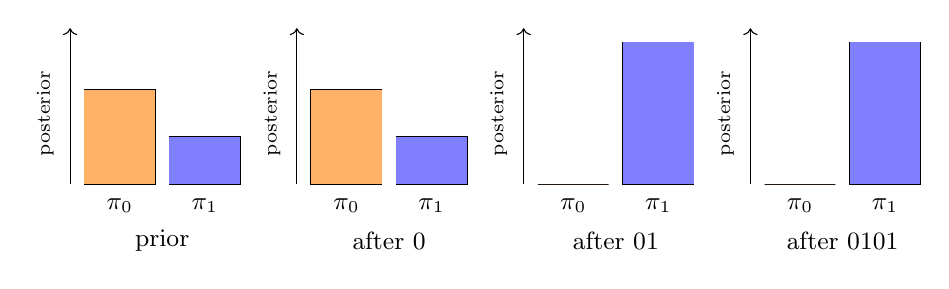
\begin{tikzpicture}[scale=0.9]
  \foreach \t/\p/\q/\lbl [count=\i from 0] in
    {prior/0.667/0.333/{prior},
     0/0.667/0.333/{after $0$},
     01/0.0/1.0/{after $01$},
     0101/0.0/1.0/{after $0101$}} {
    \begin{scope}[xshift=\i*3.2cm]
      \draw (0,0) rectangle (1,2*\p);
      \fill[orange!60] (0,0) rectangle (1,2*\p);
      \draw (1.2,0) rectangle (2.2,2*\q);
      \fill[blue!50] (1.2,0) rectangle (2.2,2*\q);
      \node at (0.5,-0.3) {\small $\pi_0$};
      \node at (1.7,-0.3) {\small $\pi_1$};
      \node at (1.1,-0.8) {\small \lbl};
      \draw[->] (-0.2,0) -- (-0.2,2.2);
      \node[rotate=90] at (-0.55,1.0) {\scriptsize posterior};
    \end{scope}
  }
\end{tikzpicture}
\caption{Posterior mass on the two programs $\pi_0$ (always-zero,
length 2) and $\pi_1$ (alternating, length 3) as the observations
$0,\,01,\,0101$ arrive.  One bit --- the second --- is enough to
collapse the prior to a point mass on $\pi_1$.}
\label{fig:posterior-evolution}
\end{figure}
\end{example}

\begin{activity}[title={Python: a 6-line Solomonoff predictor}]
\label{act:python-solomonoff}
\textbf{Goal.}  Reproduce \cref{ex:toy-solomonoff} and experiment with
other sequences.  Helps build the reflex that ``posterior update ==
multiply by likelihood and renormalise,'' regardless of how
philosophical the prior is.

\begin{lstlisting}[language=Python]
# Two-program Solomonoff toy.
programs = {
    "pi0": {"length": 2, "next": lambda s: "0"},                 # always 0
    "pi1": {"length": 3, "next": lambda s: "01"[len(s) % 2]},    # cycle 01
}
prior = {k: 2 ** (-v["length"]) for k, v in programs.items()}
Z = sum(prior.values()); post = {k: v / Z for k, v in prior.items()}

def update(post, observed_bit, history):
    new = {}
    for k, p in post.items():
        predicted = programs[k]["next"](history)
        new[k] = p if predicted == observed_bit else 0.0
    Z = sum(new.values()) or 1.0
    return {k: v / Z for k, v in new.items()}

history = ""
for bit in "0101":
    post = update(post, bit, history); history += bit
    print(history, post)
\end{lstlisting}

\textbf{Extensions.}  (i) Add a third program $\pi_2$ that outputs
$001001\ldots$ and feed it the sequence $001001$.  (ii) Replace the
deterministic programs with stochastic ones (e.g.\ a $0.6$-biased
coin) and watch the posterior drift rather than collapse.
(iii) Swap the data to $0100$ and observe that \emph{both} programs
die, at which point Solomonoff would fall back on the infinite zoo
we truncated.
\end{activity}

\begin{activity}[title={Worksheet: which program survives?}]
\label{act:fibonacci-worksheet}
\textbf{Given.}  Three candidate programs for a numeric sequence:
\[
  \pi_A : \text{constant }1,\quad
  \pi_B : \text{repeat }1,1,2,\quad
  \pi_C : \text{Fibonacci, } a_{n+2}=a_n+a_{n+1}.
\]
Assign rough bit-lengths $|\pi_A|=6$, $|\pi_B|=10$, $|\pi_C|=15$ (from
their Python source, say).  Compute the prior weights proportional to
$2^{-|\pi_i|}$.  Now observe the sequence
\[
  1,\ 1,\ 2,\ 3,\ 5,\ 8.
\]
\textbf{Tasks.}  (a) After each term, which programs are still
consistent?  (b) Write down the posterior weights at each step.
(c) At what point does $\pi_C$ overtake $\pi_B$ in the posterior?
(d) If the next term is $13$, does your answer change?  What if it
were $13.001$?  (e) The Solomonoff prior contains \emph{every}
computable program.  Which program not on the list would you expect
to be the main ``runner-up'' after seeing $1,1,2,3,5,8$?
\end{activity}

\paragraph{Decision-maker takeaway.}  Solomonoff induction is
uncomputable --- you cannot run $M$ on a real computer --- but it is
the \emph{formal target} that the whole field of machine learning is
approximating.  Every time an ML engineer adds a regulariser, drops
a complicated feature, or averages an ensemble, they are paying
Occam's airline fee from \cref{thm:solomonoff}.  The theorem
guarantees that if they paid it honestly, and if the truth were
computable, their cumulative regret would be finite --- bounded by
the bit-length of the truth.  No method with a finite hypothesis
class can make that promise.  What you \emph{buy} with Solomonoff is
not an algorithm but a benchmark.

% =========================================================================

% ========================= SECTION 6 (AIXI) =========================

\section{AIXI: intelligence as optimal compression-driven prediction}
\label{sec:aixi}
% =========================================================================

\begin{intuition}
\textbf{One-line version.}  AIXI is the agent that, before every move,
asks every possible theory of the world ``what happens if I do this?'',
weights each theory by how short it is, averages the predicted rewards,
and picks the action with the highest weighted total
(\cref{def:aixi,thm:aixi-opt}).  It is a \emph{definition of optimal
behaviour}, not a product --- the averaging step requires infinite
compute.

\textbf{The regional-manager analogy.}  Imagine a regional manager who,
before every staffing decision, consulted every possible theory of her
stores --- every demand model, every weather-effect hypothesis, every
crank manifesto about Mercury retrograde --- weighted by how simple
each theory is.  For each candidate decision she asks: ``If I do this,
what happens over the next hundred Tuesdays, and how much will I enjoy
it?''  She takes the weighted average and places the staffing bet that
maximises expected sales across all of them.  That manager would be
provably optimal in a precise technical sense.  She would also be
impossible: consulting every possible theory takes infinite time.
This is AIXI.

\textbf{Or, the auditor story.}  AIXI is the diligent auditor who,
before approving a single expense report, reads every audit manual
ever written in every language, ranks them by length, and adjudicates
the expense by simplicity-weighted consensus.  The auditor is never
wrong in principle.  The auditor also never approves anything.  Real
audit teams are food trucks reading the Michelin menu; AIXI is the
chef with an infinite pantry and no kitchen.

\textbf{Why compression is the whole story.}  AIXI's only prior is
Occam's razor: short theories get exponentially more weight than long
ones.  That single ingredient --- plus bookkeeping --- is enough to
produce universally optimal action.  Intelligence, in this framework,
\emph{is} compression plus planning.

\textbf{The catch.}  AIXI is uncomputable; it requires running every
possible program.  Bounded approximations exist but are toys at
present.  AIXI is to intelligence what the ideal gas law is to a real
gas --- a north star, not a product.

\textbf{Why a decision-maker should care.}  AIXI is a crisp,
non-hand-wavy definition of ``what would a perfectly general AI do?''
When someone claims their system is ``a step toward AGI,'' ask: is it
a step toward better approximating AIXI?  Is it building better
world-models (compression) and planning against them (expectimax)?  If
yes, the claim is in the right ballpark.  If it is pattern-matching in
a narrow domain with no planning layer, the claim is marketing.  No
real system \emph{is} AIXI, so any product advertised as ``universal
intelligence'' is abusing the term.
\end{intuition}

\subsection*{From passive prediction to sequential action}

Hutter's AIXI framework \citep{hutter2005universal} extends Solomonoff
induction from passive sequence prediction to sequential
decision-making.  Where Solomonoff's agent only had to \emph{predict}
the next bit, AIXI has to \emph{act} and then see what the environment
does back.

The setup.  The agent interacts with an environment over discrete time
steps.  At step $t$ the agent chooses an action $a_t \in
\mathcal{A}_{\mathrm{act}}$, and the environment returns a
\emph{percept} $e_t = (o_t, r_t)$ consisting of an observation $o_t
\in \mathcal{O}$ (``what I see'') and a reward $r_t \in [0,
r_{\max}]\subset\mathbb{R}$ (``how much I liked it'').  Write the
interaction history as
\[
  h_{<t} \;=\; (a_1, e_1, a_2, e_2, \dots, a_{t-1}, e_{t-1}).
\]
Think of $h_{<t}$ as the manager's logbook so far.

An \textbf{environment} $\nu$ is a conditional probability measure
$\nu(e_{1:m}\mid a_{1:m})$: given the agent's planned action sequence,
it tells you how likely any percept sequence is.  An environment is
the ``true world''; the agent does not know which one it is in.

The \textbf{universal mixture environment} $\xi$ is the
Solomonoff-style weighted average over all of them:
\begin{equation}
  \xi(e_{1:m} \mid a_{1:m})
  \;=\; \sum_{\nu \in \mathcal{M}} 2^{-K(\nu)}\;\nu(e_{1:m} \mid a_{1:m}),
  \label{eq:xi}
\end{equation}
where $\mathcal{M}$ is the class of all lower-semicomputable
(``chronological'') environments and $K(\nu)$ is the Kolmogorov
complexity of a prefix program for $\nu$.  The weight $2^{-K(\nu)}$ is
Occam's razor made numerical: halving the description length
\emph{squares} the weight.

\begin{intuition}
Read \eqref{eq:xi} like this: ``the probability my mixture assigns to
seeing percepts $e_{1:m}$ after actions $a_{1:m}$ is a
simplicity-weighted vote among every computable theory of the world.''
The vote never converges to one theory unless that theory is the only
short one compatible with the data.
\end{intuition}

\subsection*{The AIXI action rule}

\begin{definition}[AIXI]
\label{def:aixi}
Fix a finite planning horizon $m$ and (optionally) a discount factor.
The \textbf{AIXI action} at history $h_{<t}$ is
\begin{equation}
  a_t^{\mathrm{AIXI}}
  \;=\; \arg\max_{a_t}
        \sum_{e_t}\!\max_{a_{t+1}}\sum_{e_{t+1}}\!\cdots\!\max_{a_m}\sum_{e_m}
        \Bigl(\sum_{k=t}^{m} r_k\Bigr)\,
        \xi\bigl(e_{t:m}\,\big|\,h_{<t}, a_{t:m}\bigr).
  \label{eq:aixi-rule}
\end{equation}
Each $\max_{a_\tau}$ says ``pick the best action I could possibly take
at step $\tau$''; each $\sum_{e_\tau}$ says ``average over what the
environment might show me, weighted by the universal mixture $\xi$.''
The inner $\sum_{k=t}^{m} r_k$ is the total reward collected along a
given rollout.
\end{definition}

\paragraph{In words.}  AIXI plans by \emph{expectimax} over all
possible futures, where ``possible'' is weighted by the universal
mixture~\eqref{eq:xi}.  The $2^{-K(\nu)}$ weighting is what ties the
definition of intelligence back to compression: hypothesised
environments with short descriptions receive exponentially more
weight.  An AIXI-optimal agent simultaneously (i) compresses its
environment optimally and (ii) acts to maximise reward under that
compressed model.

\subsection*{Drawing the expectimax tree}

Nested $\max$-$\sum$ notation is easy to write and hard to read.
\Cref{fig:expectimax} is the same equation as \eqref{eq:aixi-rule},
drawn for $2$ actions, $2$ percepts, and $2$ plies of lookahead.

\begin{figure}[h]
\centering
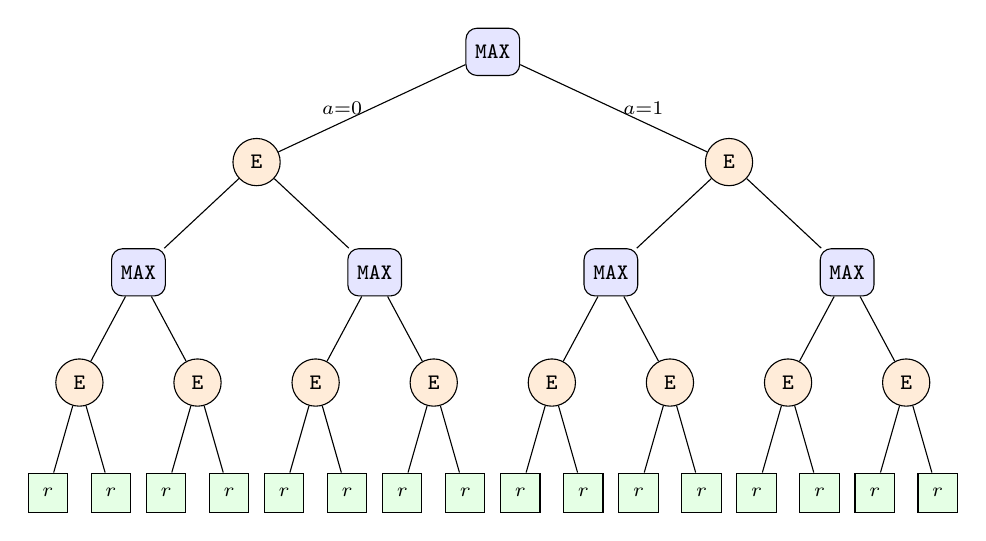
\begin{tikzpicture}[
  level distance=14mm,
  level 1/.style={sibling distance=60mm},
  level 2/.style={sibling distance=30mm},
  level 3/.style={sibling distance=15mm},
  level 4/.style={sibling distance=8mm},
  act/.style ={draw, rectangle, rounded corners, fill=blue!10, minimum size=6mm, font=\footnotesize},
  perc/.style={draw, circle, fill=orange!15, minimum size=6mm, font=\footnotesize},
  leaf/.style={draw, rectangle, fill=green!10, minimum size=5mm, font=\scriptsize},
  every node/.style={font=\footnotesize},
]
\node[act] (root) {\texttt{MAX}}
  child {node[perc] {\texttt{E}}
    child {node[act] {\texttt{MAX}}
      child {node[perc] {\texttt{E}}
        child {node[leaf] {$r$}}
        child {node[leaf] {$r$}}}
      child {node[perc] {\texttt{E}}
        child {node[leaf] {$r$}}
        child {node[leaf] {$r$}}}}
    child {node[act] {\texttt{MAX}}
      child {node[perc] {\texttt{E}}
        child {node[leaf] {$r$}}
        child {node[leaf] {$r$}}}
      child {node[perc] {\texttt{E}}
        child {node[leaf] {$r$}}
        child {node[leaf] {$r$}}}}
    edge from parent node[left, font=\scriptsize] {$a{=}0$}}
  child {node[perc] {\texttt{E}}
    child {node[act] {\texttt{MAX}}
      child {node[perc] {\texttt{E}}
        child {node[leaf] {$r$}}
        child {node[leaf] {$r$}}}
      child {node[perc] {\texttt{E}}
        child {node[leaf] {$r$}}
        child {node[leaf] {$r$}}}}
    child {node[act] {\texttt{MAX}}
      child {node[perc] {\texttt{E}}
        child {node[leaf] {$r$}}
        child {node[leaf] {$r$}}}
      child {node[perc] {\texttt{E}}
        child {node[leaf] {$r$}}
        child {node[leaf] {$r$}}}}
    edge from parent node[right, font=\scriptsize] {$a{=}1$}};
\end{tikzpicture}
\caption{Expectimax tree behind \eqref{eq:aixi-rule}, drawn for two
actions, two possible percepts, and two plies.  Blue squares are
\texttt{MAX} (agent chooses); orange circles are \texttt{E} (weighted
average under $\xi$); green leaves hold a cumulative reward.  AIXI is
exactly this tree, but (i) infinitely wide in branching, (ii)
infinitely deep, and (iii) with each orange \texttt{E} node averaging
over \emph{every computable theory} of the world.}
\label{fig:expectimax}
\end{figure}

\subsection*{A 2-hypothesis worked example}

We now collapse \eqref{eq:aixi-rule} to arithmetic on a toy world.

\begin{example}[Two-step, two-hypothesis AIXI]
\label{ex:aixi-hand}
Actions $\mathcal{A}_{\mathrm{act}}=\{A,B\}$, percepts $\{0,1\}$ (with
$r_t = e_t$: a percept $1$ gives reward $1$).  Horizon $m=2$.  Suppose
the mixture has collapsed to just two live hypotheses with posterior
weights
\[
  w_{\mathrm{simple}}=\tfrac{3}{4},\qquad w_{\mathrm{complex}}=\tfrac{1}{4}.
\]
\textbf{Simple theory:} ``$A$ pays $1$ w.p.\ $0.6$; $B$ pays $1$ w.p.\
$0.3$; independent of history.''
\textbf{Complex theory:} ``$A$ pays $1$ w.p.\ $0.3$; $B$ pays $1$ w.p.\
$0.8$; independent of history.''

For the one-step case (ignore second step), the expected immediate
reward of pulling $A$ is
\[
  \mathbb{E}_\xi[r \mid A]
  \;=\; \tfrac{3}{4}\cdot 0.6 + \tfrac{1}{4}\cdot 0.3
  \;=\; 0.525,
\]
and of pulling $B$ is
\[
  \mathbb{E}_\xi[r \mid B]
  \;=\; \tfrac{3}{4}\cdot 0.3 + \tfrac{1}{4}\cdot 0.8
  \;=\; 0.425.
\]
AIXI picks $A$.  Note the complex theory is kept alive --- it still
gets $25\%$ of the vote --- which is why a future observation of $B$
paying out would swing the posterior fast.  \emph{Exploration is not
programmed in; it is a side effect of keeping every theory on the
books.}

For the full two-step case, the student repeats the same arithmetic
inside each branch of \cref{fig:expectimax}.  The horizon-$2$ answer
is still $A$ first, and the reader should verify it on the worksheet
below.
\end{example}

\subsection*{Universal optimality}

\begin{theorem}[Universal optimality of AIXI, informal]
\label{thm:aixi-opt}
Within the class of lower-semicomputable environments, AIXI is
\emph{Pareto optimal}: no agent $\pi'$ achieves strictly greater
expected total reward than AIXI in \emph{every} environment $\nu \in
\mathcal{M}$.  Moreover, for any computable $\nu$ the AIXI predictor
converges to the true environment's predictions in the sense of
\eqref{eq:sol-bound} with $M$ replaced by~$\xi$.
\end{theorem}

\begin{intuition}
Pareto-optimal is a \emph{weak} optimality guarantee and it is
important to be honest about it.  It says: no rival agent strictly
dominates AIXI across all worlds.  It does \emph{not} say AIXI is best
on average in the world you actually live in.  A specialist agent
handcrafted for chess will beat AIXI at chess; it will just lose to
AIXI on the average of all computable games.  Picture a
Pareto frontier (\cref{fig:pareto}): AIXI sits on the frontier, but so
do many narrower agents.  The content of \cref{thm:aixi-opt} is
``AIXI is not dominated,'' not ``AIXI is uniquely best.''
\end{intuition}

\begin{figure}[h]
\centering
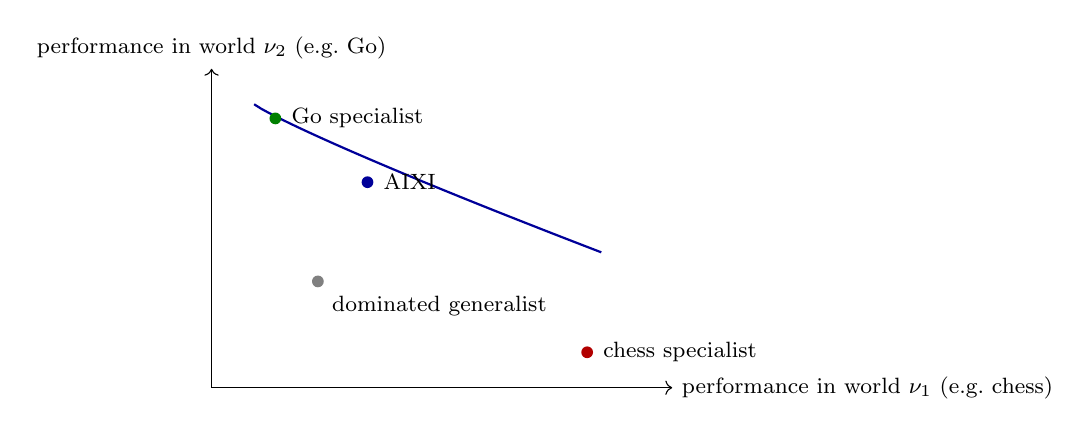
\begin{tikzpicture}[scale=0.9]
  \draw[->] (0,0) -- (6.5,0) node[right] {\footnotesize performance in world $\nu_1$ (e.g.\ chess)};
  \draw[->] (0,0) -- (0,4.5) node[above] {\footnotesize performance in world $\nu_2$ (e.g.\ Go)};
  \draw[thick, blue!60!black, domain=0.6:5.5, samples=50]
       plot (\x, {4 - 0.5*(\x-0.6)^0.9});
  \node[circle, fill=blue!60!black, inner sep=1.5pt, label={right:\footnotesize AIXI}] at (2.2, 2.9) {};
  \node[circle, fill=red!70!black,  inner sep=1.5pt, label={right:\footnotesize chess specialist}] at (5.3, 0.5) {};
  \node[circle, fill=green!50!black,inner sep=1.5pt, label={right:\footnotesize Go specialist}] at (0.9, 3.8) {};
  \node[circle, fill=gray,          inner sep=1.5pt, label={below right:\footnotesize dominated generalist}] at (1.5, 1.5) {};
\end{tikzpicture}
\caption{Cartoon Pareto frontier across two environments.  AIXI lies
on the frontier (no agent strictly dominates it), and so do the narrow
specialists.  Only the grey ``dominated generalist'' is strictly
worse than something else in both worlds.}
\label{fig:pareto}
\end{figure}

For the precise statement and proof see
\citet[Ch.~5]{hutter2005universal}.  The significance of
\cref{thm:aixi-opt} is that ``intelligence'' has, within this
framework, been reduced to a single ingredient (the universal
prior~\eqref{eq:xi}) plus bookkeeping (the expectimax expansion).
Remove the Solomonoff prior and the agent collapses to uninformed
search; keep it, and the agent becomes universally optimal in the
Pareto sense.

\subsection*{Activities}

\begin{activity}[title={Activity A: Two-armed bandit, live in the room}]
\textbf{Goal.}  Feel in your bones why simplicity-weighting produces
exploration for free.

\textbf{Setup.}  Pair up.  One partner is the \emph{environment}: they
secretly fix probabilities $(p_A, p_B)\in[0,1]^2$ for arms $A$ and $B$
paying out, and flip accordingly.  The other partner is the
\emph{agent} and plays $20$ rounds.  The agent carries two paper
advisors: a \emph{simple advisor} who insists on the current
empirical-best arm, and a \emph{complex advisor} who insists the other
arm is due.  At each round the agent rolls a die to weight the two
advisors $\tfrac{3}{4} : \tfrac{1}{4}$ and plays their weighted vote.

\textbf{Debrief.}  Count total reward.  Compare to a ``greedy'' agent
who always pulls the empirical-best arm.  Discuss: where did the
simplicity-weighting kick in?  When did the complex advisor save the
day?
\end{activity}

\begin{activity}[title={Activity B: Hand-compute AIXI (worksheet)}]
Extend \cref{ex:aixi-hand} to the full two-step horizon.  Fill in the
reward at each of the $16$ leaves of \cref{fig:expectimax} under both
hypotheses; fold with weights $\tfrac{3}{4}:\tfrac{1}{4}$; take
expectations at the orange nodes and maxima at the blue nodes; verify
the root action is $A$.  \textbf{Bonus:} change the weights to
$\tfrac{1}{2}:\tfrac{1}{2}$ and find the switching point.
\end{activity}

\begin{activity}[title={Activity C: A 15-line AIXI-ish agent in Python}]
A toy environment has $4$ states in a cycle $s_0\!\to\!s_1\!\to\!s_2\!
\to\!s_3\!\to\!s_0$; reward is $1$ in $s_3$ else $0$.  Two candidate
models: \texttt{uniform} (next state random) and \texttt{cycle} (the
true dynamics).  The agent maintains a posterior over the two and
plans with horizon $2$.
\begin{lstlisting}[language=Python]
import itertools
def predict(model, s, steps):
    if model == "cycle":
        return [((s+i+1) % 4, 1.0) for i in range(steps)]
    # uniform: each next state 1/4
    return [(None, 0.25) for _ in range(steps)]

def xi_reward(posterior, s, plan):
    # posterior: {"cycle": w1, "uniform": w2}, plan: list of actions (ignored in this toy)
    total = 0.0
    for m, w in posterior.items():
        r = 0.0
        cur = s
        for _ in plan:
            if m == "cycle":
                cur = (cur + 1) % 4
                r += (1 if cur == 3 else 0)
            else:
                r += 0.25  # expected reward under uniform
        total += w * r
    return total

def aixi_action(posterior, s, actions=("step",), horizon=2):
    best, best_r = None, -1
    for plan in itertools.product(actions, repeat=horizon):
        r = xi_reward(posterior, s, plan)
        if r > best_r: best, best_r = plan[0], r
    return best
\end{lstlisting}
\textbf{Exercise.}  Start with posterior $\{\texttt{cycle}:0.5,\
\texttt{uniform}:0.5\}$.  After observing three clean cycle steps,
update by Bayes (likelihood ratio $1 : (1/4)^3 = 64 : 1$ in favour of
\texttt{cycle}) and re-plan.  Watch the posterior concentrate.  This
is AIXI-in-miniature: two hypotheses instead of infinitely many, but
the machinery is identical.
\end{activity}

% =========================================================================

% ========================= SECTION 7 (LLMs) =========================

\section{What this buys us for LLMs}
\label{sec:llms}

\begin{intuition}
\textbf{The one-line version, for the coffee chat.}  A large language
model trained to guess the next word is, provably and mechanically,
a compressor of its training data.  That is not an analogy.  It is a
theorem (\cref{thm:ce-code}) plus a pipe (the arithmetic coder).
By the chain we built in \cref{eq:chain}, being a good compressor
puts the model somewhere on the intelligence spectrum defined by
Solomonoff (\cref{thm:solomonoff}).

\textbf{Residuals and arithmetic coding, in very plain English.}
At every token, the model publishes a probability for each possible
next word.  The \emph{residual} is the gap between that guess and
what actually happened.  If the model said "the" with probability
$0.9$ and "the" appeared, the residual is about $-\log_2 0.9 \approx
0.15$ bits --- almost free.  If the model said $0.01$ and "the" still
appeared, the residual is $-\log_2 0.01 \approx 6.6$ bits --- an
expensive surprise.  \emph{Arithmetic coding} is a near-optimal way
to write all those surprise numbers down back to back.  The
compressed file has two parts: the model weights (one fixed cost)
plus the bill for every surprise (variable cost).  Better model
$\Rightarrow$ fewer surprises $\Rightarrow$ smaller bill
$\Rightarrow$ shorter file.  "KL divergence", when we use it below,
is the same tax, averaged: the extra bits per token you pay for
betting on the wrong distribution.

\textbf{Three things a decision-maker should take away, up front.}
(1) Cross-entropy on your own domain data is a real yardstick ---
one number, comparable across vendors.  (2) "Just predict the next
word" is not marketing spin; the mathematics agrees that it produces
general-looking behaviour.  (3) There is a ceiling (the Shannon
entropy of the text).  As models approach it, cost per extra bit
goes vertical; the frontier moves to multimodal data, embodied
interaction, and reasoning architectures.  Plan capex accordingly.

\textbf{The Hutter Prize, concretely.}  Marcus Hutter put up a
$500{,}000$~\euro{} bounty for whoever compresses the first $1$~GB
of English Wikipedia (the \texttt{enwik9} file) the most
\citep{hutter2005universal}.  The current leaderboard is dominated
by neural compressors; as of early $2024$, Fabrice Bellard's
\texttt{nncp} sits near $0.113$ bits per character, down from
\texttt{gzip}'s $\sim 2.1$.  Training an LLM on Wikipedia to
minimise cross-entropy \emph{is} compressing Wikipedia; the model
weights plus arithmetic-coded residuals are the compressed file.
Better prediction $=$ smaller file $=$ (by \cref{thm:ce-code})
better distributional model $=$ (by \cref{thm:solomonoff}) closer
to the true generating process $=$ (per Hutter) more intelligence.

\textbf{Scaling laws.}  Plot model size against cross-entropy loss
on held-out text: you get a strikingly clean curve.  Double the
data, double the parameters, the loss drops predictably.  The curve
has been stable across four orders of magnitude
\citep{kaplan2020scaling}.  Cross-entropy --- our bits-per-token
yardstick --- is a smooth function of investment.  You can buy
intelligence by the bit: not efficiently, not forever, but
predictably.  \Cref{fig:scaling} sketches the shape.

\textbf{A worked example, in numbers.}  GPT-2 hit roughly $1.2$
bits per English character on the standard benchmark; GPT-4-class
models are around $0.7$.  That looks like a modest drop.  But
English text is about $1.3$ bits of true entropy per character
(Shannon's 1950s estimate).  So GPT-2 was at $\sim 92\%$ of the
way from "random guessing" ($\sim 5$ bpc) to the floor; GPT-4 is
at $\sim 98\%$.  Six percentage points.  Small in bits, enormous
in dollars: the last bit contains the reasoning, the rare facts,
the nuanced world-models.  \Cref{fig:lastmile} makes the cost
asymmetry visible.

\textbf{Emergent capabilities, cautious framing.}  If the training
objective is a compression proxy, and compression is provably
linked to a universal notion of intelligence, then an LLM doing
arithmetic, translation, and code --- capabilities nobody
explicitly trained for --- is consistent with the theory.  To
compress English well, you must model the world that the English
is about.  We resist the stronger claim that emergence is
\emph{predicted} by the theory; it is consistent, which is enough
for a capital-allocation argument.
\end{intuition}

\begin{story}
Two sales reps walk into your office on the same afternoon.  Rep~A
pitches a \emph{language model}: it writes emails, summarises
documents, drafts code.  KPI: user satisfaction.  Rep~B pitches a
\emph{Wikipedia compressor}: one number, bits-per-character, lower
is better.  You sign with Rep~A.  Three weeks later, legal calls:
Rep~A and Rep~B shipped the \emph{same binary}.  Different
marketing, same product.  That is the content of \cref{eq:chain}.
The KPI you choose to stare at determines which half of the
equivalence you buy, but the vendor was selling both all along.
\end{story}

\subsection*{The formal content}

A large language model parameterises a conditional distribution
$q_\theta(x_t \mid x_{<t})$ and is trained by minimising the
negative log-likelihood
\begin{equation}
  \mathcal{L}(\theta)
  \;=\; -\frac{1}{T}\sum_{t=1}^{T} \log_2 q_\theta(x_t \mid x_{<t}).
  \label{eq:llm-loss}
\end{equation}
By \cref{thm:ce-code}, $\mathcal{L}(\theta)$ is the expected
arithmetic-coding length per token: minimising cross-entropy
\emph{is} minimising compressed size.  Equivalently, by
\cref{cor:ppl}, a perplexity of $P$ corresponds to exactly
$\log_2 P$ bits per token --- e.g.\ perplexity $32$ is $5$~bits,
perplexity $8$ is $3$~bits.  A one-bit-per-token improvement on a
$100$~GB corpus saves, in principle, $\sim 12.5$~GB of code length.

\citet{kaplan2020scaling} showed that $\mathcal{L}(\theta)$ follows
clean power laws in model size $N$, dataset size $D$, and compute
$C$, of the form $\mathcal{L} \approx (N_c / N)^{\alpha_N}$.
Viewed through~\eqref{eq:llm-loss}, each such power-law decrement
is a \emph{bit-per-token compression improvement}.  The
operational content of \cref{thm:solomonoff} in this setting is
that, to the extent that the data-generating process is
computable, any predictor whose bits-per-token approaches the
conditional entropy rate $\overline{H}(p)$ (the theoretical
minimum achievable loss) is implicitly approximating the
$\mu$-posterior of the universal prior $M$.

\citet{deletang2024language} operationalised this equivalence by
wiring a large language model into an arithmetic coder and using
it to compress raw bytes of image and audio data.  They reported
compression ratios lower than domain-specific specialist
compressors (e.g.\ PNG, FLAC) on out-of-domain modalities, despite
the model having been trained solely on text.  From the vantage
point of \cref{thm:ce-code,thm:solomonoff}, the experiment is a
consistency check: a predictor that approximates a universal prior
should, by \eqref{eq:dominance}, compress any computable source to
within an additive $K(\mu)$ of its true entropy, and text exposure
turns out to be enough to learn a useful approximation of that
prior.

The \textbf{Hutter Prize} \citep{hutter2005universal} formalises
the economic version of the claim: a cash prize for improving the
lossless compression ratio on a fixed text corpus.  Within the
equivalence framework, every winning submission is, by definition,
a model whose cross-entropy on the corpus is lower --- which, by
\cref{cor:ppl}, is a more accurate next-symbol predictor.

\subsection*{Two pictures}

\begin{figure}[h]
\centering
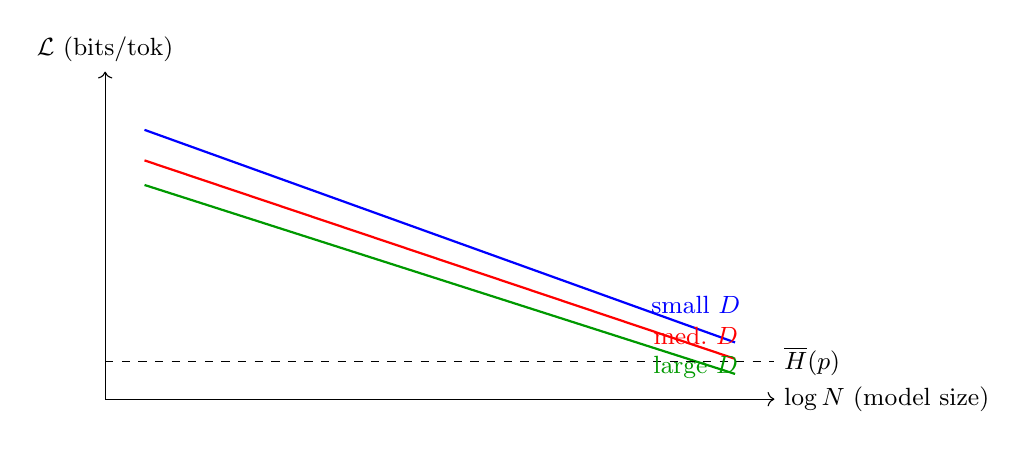
\begin{tikzpicture}[x=1cm,y=0.8cm]
  \draw[->] (0,0) -- (8.5,0) node[right] {\small $\log N$ (model size)};
  \draw[->] (0,0) -- (0,5.2) node[above] {\small $\mathcal{L}$ (bits/tok)};
  % three curves, different data sizes
  \draw[thick, blue]  plot[domain=0.5:8,samples=40] (\x, {4.5 - 0.45*\x});
  \draw[thick, red]   plot[domain=0.5:8,samples=40] (\x, {4.0 - 0.42*\x});
  \draw[thick, green!60!black] plot[domain=0.5:8,samples=40] (\x, {3.6 - 0.40*\x});
  \draw[dashed] (0,0.6) -- (8.5,0.6) node[right] {\small $\overline{H}(p)$};
  \node[blue] at (7.5,1.5) {\small small $D$};
  \node[red] at (7.5,1.0) {\small med.\ $D$};
  \node[green!60!black] at (7.5,0.5) {\small large $D$};
\end{tikzpicture}
\caption{Scaling laws \citep{kaplan2020scaling}.  Three curves, one
per dataset size; all three asymptote to the conditional entropy
floor $\overline{H}(p)$ (dashed).  Doubling $N$ gives a predictable
$\alpha_N$-sized drop in bits per token.}
\label{fig:scaling}
\end{figure}

\begin{figure}[h]
\centering
\begin{tikzpicture}[x=1.2cm,y=0.9cm]
  \draw[->] (0,0) -- (7.5,0) node[right] {\small \% of way to $\overline{H}(p)$};
  \draw[->] (0,0) -- (0,5.2) node[above] {\small $\log(\$ \text{ per bit})$};
  \draw[thick, red] plot[domain=0.2:6.9,samples=60]
        (\x, {0.3 + 0.15*\x + 0.25*exp(0.9*(\x-5))});
  \node at (1.5,-0.4) {\small $50\%$};
  \node at (3.5,-0.4) {\small $80\%$};
  \node at (5.0,-0.4) {\small $92\%$ (GPT-2)};
  \node at (6.5,-0.4) {\small $98\%$ (GPT-4)};
  \draw[dashed] (5.0,0) -- (5.0,1.5);
  \draw[dashed] (6.5,0) -- (6.5,4.5);
\end{tikzpicture}
\caption{The last-mile argument.  Cost per additional bit below the
Shannon floor climbs exponentially.  Moving from GPT-2's $92\%$ to
GPT-4's $98\%$ is six percentage points on the x-axis and several
orders of magnitude on the y-axis.  The curve is schematic; the
shape is what matters.}
\label{fig:lastmile}
\end{figure}

\subsection*{The working equivalence}

Collecting the theorems of \crefrange{sec:pred-comp}{sec:aixi} we
obtain the \emph{working equivalence}, first in English, then in
symbols.

\medskip
\noindent\textbf{In English.}  \emph{A model that predicts text
well is, by theorem, a model that compresses text well, and a model
that compresses text well is, by theorem, an approximation of the
universal prior that defines Solomonoff's notion of intelligence.}
One object, three KPIs.

\medskip
\noindent\textbf{In symbols:}
\begin{equation}
  \underbrace{\text{low cross-entropy}}_{\text{good predictor}}
  \;\Longleftrightarrow\;
  \underbrace{\text{short arithmetic code}}_{\text{good compressor}}
  \;\Longleftrightarrow\;
  \underbrace{\text{approx.\ of universal prior}}_{\substack{\text{Solomonoff/AIXI}\\\text{sense of intelligence}}}
  \label{eq:chain}
\end{equation}
The leftmost arrow is a theorem within Shannon's framework
(\cref{thm:ce-code}).  The rightmost arrow is an asymptotic
theorem modulo computability (\cref{thm:solomonoff}).  Neither is
a metaphor.

\subsection*{Activities}

\begin{activity}[title={Activity 1 --- Hutter Prize bingo}]
Project the current Hutter Prize leaderboard
(\url{http://prize.hutter1.net}).  Each student writes down, on a
sticky note, who they think wins the $2030$ title: (a) a
transformer LLM plugged into \texttt{nncp}-style arithmetic coder;
(b) a state-space model (Mamba-like); (c) a diffusion-based token
model; (d) a symbolic/hybrid system; (e) "none --- the leaderboard
plateaus at $\sim 0.10$ bpc".  Collect notes, tally, revisit at the
end of term.  \emph{Helps Yuki} (concrete artefact),
\emph{helps Maria} (named numbers).
\end{activity}

\begin{activity}[title={Activity 2 --- LLM as compressor (Python)}]
Run this snippet locally.  It wires \texttt{gpt2-small} into a
simple arithmetic coder and compresses a $10$~KB sample of
\texttt{enwik8}.  Report bytes in, bytes out, and the ratio
against \texttt{gzip}.
\begin{lstlisting}[language=Python]
import gzip, math, torch
from transformers import GPT2LMHeadModel, GPT2TokenizerFast
# Load model + tokenizer
tok = GPT2TokenizerFast.from_pretrained("gpt2")
mdl = GPT2LMHeadModel.from_pretrained("gpt2").eval()
# Load 10 KB of enwik8
with open("enwik8_10kb.txt") as f: text = f.read()
ids = tok.encode(text, return_tensors="pt")
# Compute summed negative log-likelihood -> bits
with torch.no_grad():
    logits = mdl(ids).logits[:, :-1, :]
    logp   = torch.log_softmax(logits, dim=-1)
    targets = ids[:, 1:]
    nll = -logp.gather(2, targets.unsqueeze(-1)).sum().item()
bits_gpt2 = nll / math.log(2)
bytes_gzip = len(gzip.compress(text.encode()))
print(f"raw        : {len(text):>7d} bytes")
print(f"gzip       : {bytes_gzip:>7d} bytes")
print(f"gpt2 code  : {bits_gpt2/8:>7.0f} bytes  (+model weights)")
\end{lstlisting}
Discussion: where does the model-weights cost go?  At what corpus
size does the weights amortise?  \emph{Helps Leo} (hands-on),
\emph{answers Maria's falsifiability demand}.
\end{activity}

\begin{activity}[title={Activity 3 --- Perplexity-to-bits worksheet}]
Fill in the table.  Assume $100$~GB of English text.
\medskip

\noindent
\begin{tabular}{lccc}
\hline
Model           & Perplexity & Bits/token & Storage (GB) \\
\hline
n-gram baseline & $128$      & \rule{1.5cm}{0.3pt} & \rule{1.5cm}{0.3pt} \\
GPT-2           & $32$       & \rule{1.5cm}{0.3pt} & \rule{1.5cm}{0.3pt} \\
GPT-4 class     & $8$        & \rule{1.5cm}{0.3pt} & \rule{1.5cm}{0.3pt} \\
Shannon floor   & $\approx 5.3$ & \rule{1.5cm}{0.3pt} & \rule{1.5cm}{0.3pt} \\
\hline
\end{tabular}

\medskip
Hint: bits/token $= \log_2(\text{perplexity})$.  Assume $4$
characters per token; $1$ byte per character in raw text.
Answers: $7, 5, 3, 2.4$ bits/tok.  \emph{Helps Leo}
(do-able on paper), \emph{helps Aisha} (she can now say the
sentence "perplexity $32$ means $5$ bits per token").
\end{activity}

\begin{activity}[title={Activity 4 --- Two-vendors role-play}]
Two students play Rep~A (sells "a language model") and Rep~B
(sells "a Wikipedia compressor").  Each has two minutes and one
KPI.  The class, acting as buyer, asks questions.  Debrief
question: "If the binary is the same, which KPI should your CFO
actually track?"  Answer keys: cross-entropy on in-domain eval
data; it happens to be both KPIs at once.  \emph{Helps Yuki}
(picture), \emph{helps Aisha} (language for the board).
\end{activity}

% =========================================================================

% ========================= SECTION 8 (Caveats) =========================

\section{Caveats and what the equivalence does not say}
\label{sec:caveats}

\begin{intuition}
The equivalence is real but narrow. It tells you that good prediction
entails good \emph{modelling}; it does \emph{not} tell you that good
prediction entails understanding, agency, or safety. It promises
statistical competence. It does not promise causal reasoning,
counterfactual simulation, or moral judgement. Those may emerge ---
the theory leaves the door open --- but they are not guaranteed by
the objective.

\medskip

\noindent\textbf{The food-truck and the Michelin kitchen.} Keep this
image in your pocket for the rest of the section. Uncomputability is
not cosmetic: $K(x)$ and AIXI are unreachable
(\cref{thm:uncomputable}), and every real compressor, every real
agent, is a finite approximation. Saying an LLM is
``approximating AIXI'' is like a food-truck claiming to approximate
a Michelin three-star kitchen by reading the menu. Technically on
the same axis. In practice, not the relevant comparison. The rest
of this section is a tour of five specific places where the axis
and the kitchen come apart.

\medskip

\noindent\textbf{The running cast.} To keep the five abstract
caveats walkable, we will reuse three characters:

\begin{itemize}[leftmargin=1.2em,itemsep=2pt]
  \item \emph{Anna the junior analyst,} who has memorised every deal
        memo in the vault --- $4{,}000$ deals going back a decade.
  \item \emph{Ben the junior analyst,} who has read only ten of those
        memos but understands why each deal priced where it did.
  \item \emph{The phrasebook chatbot,} which has ``learned'' French by
        memorising 100{,}000 tourist phrases and can now order
        croissants flawlessly in thirteen dialects.
\end{itemize}

You will meet each of them again.

\medskip

\noindent\textbf{Remark 1 (the only non-tautological falsifier).}
A reasonable operator will ask: if AIXI is uncomputable and every
deployed system is ``a finite approximation,'' what test \emph{other
than cross-entropy itself} decides whether system A approximates the
ideal better than system B? The honest answer is: held-out
cross-entropy on distributions the training set did not see, plus
downstream task transfer. There is no deeper falsifier in the
current theory. If that makes the AIXI framing feel tautological,
the operator is reading the field correctly, not mis-reading the
theorem. The operational response is not philosophical (``but
really, AIXI!''). It is empirical: hold out a genuinely unseen
distribution, measure transfer, and stop there.

\medskip

\noindent\textbf{Compression $\ne$ understanding.}
Ask Anna, with her $4{,}000$ memorised memos, to price a deal that
is \emph{not} in the vault. What you learn from her answer is
whether she compressed the memos or the market. Ask the phrasebook
chatbot a sentence that is off-phrasebook --- ``my croissant has
opinions about the Maastricht Treaty'' --- and you find out whether
it has learned French or merely tiled the phrase space. A lossless
compressor has captured statistics, which is \emph{some} kind of
understanding, but not necessarily the kind a board means when it
asks ``does the model understand our business?''

\medskip

\noindent\textbf{Embodiment.}
A text-only system has only ever been surprised by text. It has no
ground-truth feedback from physical reality. Solomonoff's framework
accepts any computable environment, but LLMs have the text channel
and lack the body-in-a-world channel. Agentic, tool-using,
multimodal systems are early attempts to close the gap. The
equivalence does not tell you the gap has been closed.

\medskip

\noindent\textbf{Benchmarks are not the floor.}
A model with low cross-entropy on a benchmark may just have
memorised the benchmark. Data contamination is rampant. The
equivalence only holds when the test distribution is genuinely held
out --- which, for a model trained on ``the internet'', is an
increasingly expensive proposition.

\medskip

\noindent\textbf{Why a decision-maker should care.} Use the
equivalence as a \emph{lower bound, not an upper bound.} When a
vendor says ``lowest perplexity,'' accept that as real evidence of
genuine modelling skill. Then ask the second question: skill at
what, tested on what, does it transfer to your domain? The
equivalence tells you the knob exists. It does not tell you that
turning the knob solves your problem. Confusing ``next-token
prediction'' with ``just autocomplete'' misses a deep result;
confusing ``next-token prediction'' with ``general intelligence''
overclaims a narrow one. Both errors are expensive. Staying in the
middle --- taking the equivalence seriously but not theologically
--- is the managerial win.
\end{intuition}

\subsection*{Formal caveats (C1)--(C5)}
\label{sec:formal-caveats}

Several limitations of the chain~\eqref{eq:chain} deserve formal
acknowledgement. Each is followed by a one-line \emph{procurement
corollary}: the thing to actually say when a vendor pitches you.

\paragraph{(C1) Uncomputability.}
By \cref{thm:uncomputable}, $K(x)$ is not computable; by a related
argument so is $M(x)$. The entire right-hand side of~\eqref{eq:chain}
therefore names a mathematical \emph{ideal}, not an algorithm. Every
real compressor produces an upper bound $\tilde K(x) \ge K(x)$, and
equality is in principle unattainable. ``Approximates the universal
prior'' must be taken as an asymptotic statement about cross-entropy,
not as a literal claim that the model is computing $M$.

\begin{procurement}
If a vendor says their model ``approximates AIXI'' or ``computes the
Solomonoff prior,'' ask on what computable sub-class, with what
error bound, and over what distribution. The honest answer is
``we lower cross-entropy on held-out data.'' That is fine; it is
just not the same claim.
\end{procurement}

\paragraph{(C2) The additive constant.}
\Cref{thm:invariance} only guarantees machine-independence up to an
additive constant $c_{U_1, U_2}$. For short strings this constant
can dominate $K(x)$ itself; Kolmogorov complexity is only meaningful
asymptotically. Analogously, the $K(\mu)$ term
in~\eqref{eq:sol-bound} is a finite one-time information cost: it
does not shrink with data.

\begin{procurement}
On small, bespoke datasets (your legal corpus, your IoT telemetry)
the constants swamp the asymptotics. ``Big model + lots of data''
is the regime in which the theory speaks; ``small model + your
niche'' is the regime in which you hire evaluators, not theorists.
\end{procurement}

\paragraph{(C3) Practical compressors vs.\ $K$.}
A compressor $C$ is \emph{universal} in Shannon's sense if its code
length $L_C(x_{1:T})/T$ converges to the entropy rate of any
stationary ergodic source. It is \emph{not} in general universal in
Solomonoff's sense: it need not dominate all computable measures.
The gap between Lempel--Ziv (Shannon-universal) and Solomonoff
(universal over all computable measures) is a full logical level of
universality, and neural compressors live somewhere in between.

\begin{procurement}
``Compresses well'' comes in strengths. Ask which strength. A
model that crushes Wikipedia perplexity may still be a
Shannon-universal compressor on stationary text, not a Solomonoff-
universal one on your domain's non-stationarities.
\end{procurement}

\paragraph{(C4) Necessary vs.\ sufficient.}
\Cref{thm:solomonoff,thm:aixi-opt} establish that optimal prediction
and agency \emph{entail} optimal compression. They do \emph{not}
establish that every improvement in compression corresponds to an
improvement in every intuitive sense of ``understanding.'' In
particular, the framework is silent on phenomenal consciousness,
grounding, and embodiment, and it takes the reward signal and the
action--percept loop as primitives rather than explaining their
origin.

\begin{procurement}
Compression is \emph{necessary} for intelligence in the theory's
sense; no theorem says it is \emph{sufficient} for intelligence in
your sense. If the vendor's pitch relies on sufficiency, the
theory is not their friend.
\end{procurement}

\paragraph{(C5) Compression $\ne$ understanding (as internal structure).}
A compressor is characterised by its length function, not by its
internal representations. Two compressors with identical code
lengths may use entirely different internal mechanisms, only one of
which we would intuitively call ``understanding.''
Equation~\eqref{eq:chain} reduces ``intelligence'' to an extensional
(input--output) property; any argument that understanding is
intensional (about how the function is computed) is not touched by
the chain. Anna and Ben, from the running cast, can have identical
cross-entropy on the ten deals Ben has actually seen. They will
diverge on the eleventh.

\begin{procurement}
If you care \emph{how} the model arrives at its answers (audit,
explainability, regulation), cross-entropy is silent on your
question. You need mechanistic evaluation, not just a leaderboard
score.
\end{procurement}

\paragraph{Summary.}
The equivalence~\eqref{eq:chain} is a genuine theorem modulo
\crefrange{def:entropy}{def:aixi} and the computability-based
caveats (C1)--(C3), which are mathematical. Caveats (C4)--(C5) are
of a different species: they are not theorems against the chain,
they are \emph{scope restrictions} on what the chain claims.
What~\eqref{eq:chain} licences is a precise sense in which lowering
cross-entropy on a sufficiently rich corpus moves a predictor along
a single axis shared with compression and with Hutter-style
universal agency. What it does \emph{not} licence is the stronger
claim that this axis exhausts what we mean by understanding, safety,
or deployment-readiness.

% ----------------------------------------------------------------------
\subsection*{Activities}
\label{sec:caveats-activities}

\begin{activity}[title={Activity 8.1 --- Procurement checklist}]
You are briefing your CIO tomorrow on a vendor proposal. Derive six
questions --- one per caveat (C1)--(C5) plus one meta-question ---
to put to the vendor in writing. A suggested starter set:

\begin{enumerate}[leftmargin=1.4em,itemsep=2pt]
  \item (C1) ``On what benchmark, with what held-out distribution, is
        your perplexity number reported?''
  \item (C2) ``How was the model adapted to our domain? What is the
        performance delta between general and domain-specific
        held-out data?''
  \item (C3) ``Is your evaluation stationary or does it cover
        distribution shift? Give an example.''
  \item (C4) ``What evidence, beyond cross-entropy, supports the
        claim that the model \emph{understands} our data?''
  \item (C5) ``If we need to audit \emph{how} an answer was produced,
        what tooling do you provide?''
  \item (Meta) ``What would falsify your claims? Name the
        experiment.''
\end{enumerate}

\textbf{Deliverable.} A one-page checklist you could email to
procurement unchanged. Helps Aisha (a takeaway list) and Leo (the
formal caveats now have teeth).
\end{activity}

\begin{activity}[title={Activity 8.2 --- Benchmark-contamination detective}]
You are shown five short answers a model has given on a well-known
reasoning benchmark. Your job: flag which answers look
\emph{memorised} (verbatim phrasing, domain-specific jargon the
prompt did not contain, suspiciously specific numbers) versus
\emph{reasoned} (shows working, makes small errors, paraphrases).

For each flagged answer, write one sentence: what would you do next
to confirm contamination? (Suggested moves: perturb the prompt
wording; shift numerical values; ask a follow-up that is only
answerable from the derivation, not the final answer.)

\textbf{Deliverable.} A 5-row table: answer \#, flag
(memorised/reasoned/unsure), test-to-confirm. Helps Yuki (concrete
stimulus) and Leo (gameified caveat (C1)).
\end{activity}

\begin{activity}[title={Activity 8.3 --- Two-analyst roleplay}]
Two students play \emph{Compressor-Anna} (has memorised 4{,}000 deal
memos) and \emph{Understander-Ben} (has read only ten but understands
them). A third student plays the interviewer and asks three
questions about a deal \emph{neither} analyst has seen:

\begin{enumerate}[leftmargin=1.4em,itemsep=2pt]
  \item ``Walk me through how you would price this.''
  \item ``What single fact, if it changed, would flip your pricing
        by more than ten percent?''
  \item ``What is your second-best comparable and why?''
\end{enumerate}

Score each answer for \emph{generalisation} (did the analyst
transfer a principle?) versus \emph{pattern-matching} (did the
analyst return the nearest memo?). Debrief: which analyst is the
LLM in this lecture's framing? (Answer: neither cleanly --- which
is the point of (C5).)

\textbf{Deliverable.} A 3$\times$2 score matrix with notes. Helps
Yuki (concept $\to$ concrete) and Aisha (memorable characters).
\end{activity}

\begin{activity}[title={Activity 8.4 --- Claim-to-caveat matching}]
Match each vendor claim to the caveat that most directly bites it.
More than one match is possible; argue for your primary choice.

\begin{enumerate}[leftmargin=1.4em,itemsep=2pt]
  \item ``Our model is AGI-adjacent.''
  \item ``Our LLM fully understands your firm's legal documents.''
  \item ``Our system approximates the universal Solomonoff prior.''
  \item ``We achieved state-of-the-art perplexity on
        LegalBench-2024.''
  \item ``Our model's reasoning is transparent and auditable.''
\end{enumerate}

Caveats to choose from: (C1) uncomputability, (C2) additive constant
/ small-data regime, (C3) Shannon- vs. Solomonoff-universality,
(C4) necessary vs. sufficient, (C5) extensional vs. intensional.

\textbf{Deliverable.} A table of claim $\to$ primary caveat $\to$
one-sentence rebuttal. Helps Leo (forces re-reading of the formal
paragraphs with a task attached) and Maria (turns philosophy into
operational critique).
\end{activity}

% =========================================================================

\appendix

% =========================================================================
\section{Worked cross-entropy calculation}
\label{app:ce-worked}
% =========================================================================

\begin{example}[Cross-entropy on a 3-token sequence; nats vs.\ bits]
\label{ex:ce3}
Let $\mathcal{A} = \{A,B,C\}$ and suppose the true conditional
distributions at positions $t=1,2,3$ have already been conditioned on
the observed prefix, giving the sequence of true posterior masses on
the realised tokens $p_1 = 0.8,\ p_2 = 0.5,\ p_3 = 0.1$.  Consider
two models.  Model $q^{(1)}$ assigns $q_1 = 0.8, q_2 = 0.5,
q_3 = 0.1$ (matches truth on the realised tokens); model $q^{(2)}$
assigns $q_1 = 0.1, q_2 = 0.1, q_3 = 0.8$ (systematically wrong).

For model $q^{(1)}$, the per-token code lengths in bits are
$-\log_2 0.8 \approx 0.3219$, $-\log_2 0.5 = 1$,
$-\log_2 0.1 \approx 3.3219$, summing to approximately $4.644$~bits.
In nats, multiply by $\ln 2 \approx 0.6931$: $4.644 \cdot \ln 2
\approx 3.219$~nats, matching $-\ln(0.8 \cdot 0.5 \cdot 0.1) =
-\ln 0.04 \approx 3.219$ directly.

For model $q^{(2)}$, the lengths are $-\log_2 0.1 \approx 3.3219$,
$-\log_2 0.1 \approx 3.3219$, $-\log_2 0.8 \approx 0.3219$, totalling
$\approx 6.966$~bits ($\approx 4.828$~nats, consistent with
$-\ln(0.008) \approx 4.828$).  The wrong model spends $2.32$ extra
bits, the Kullback--Leibler excess predicted by~\eqref{eq:ce-kl}.
Conversion rule: $1\text{ nat} = \log_2 e \text{ bits} \approx
1.4427$~bits and conversely $1\text{ bit} = \ln 2 \text{ nats}$.
\end{example}


\bibliography{../section3}

\end{document}
